\section{Implementation, Experimental Methodology, and Performance Evaluation}
\label{4}
This section describes the PrivSearch prototype and its reproducibility artifacts (Section~\ref{4A}), the benchmark datasets and workload design (Section~\ref{4B}), the statistical reporting protocol (Section~\ref{4C}), and the full experimental evidence: query-family and semantic benchmarks (Sections~\ref{4D}--~\ref{4E}), broader healthcare-corpus validation (Section~\ref{4F}), the direct SeaCQ-aligned comparison and broader literature-based baseline positioning (Sections~\ref{4G}--~\ref{4H}), descriptive and inferential statistics (Section~\ref{4I}), an ablation study (Section~\ref{4J}), resource-overhead and cryptographic-overhead decomposition (Sections~\ref{4K}--~\ref{4L}), scalability analysis (Section~\ref{4M}), replay-protection results (Section~\ref{4N}), WAN-style distributed-validation results (Section~\ref{4O}), and a concluding discussion (Section~\ref{4P}).
\subsection{Implementation and Reproducibility}
\label{4A}
PrivSearch is implemented as a runnable prototype (\texttt{privsearch-prototype}) integrated into an existing PureChain-backed application stack, rather than evaluated only as a paper design. The prototype implements HMAC-SHA256 trapdoor generation, AES-256-GCM encrypted posting storage, Boolean query execution for all six query families of Section~III-C, Merkle-style integrity verification over decrypted postings, and sampled RSA-style accumulator membership checks for returned documents. The operational index is realized in MongoDB with B-tree indexes over administrative attributes; encrypted payloads are stored in MinIO; blockchain anchoring and the nonce registry run against the PureChain network with Docker-managed services. All benchmark and analysis scripts, generated manuscript assets, and raw benchmark run logs are retained in the project repository and are sufficient to reproduce every table and figure reported in this section; a complete artifact availability statement, including reproduction commands and a manifest of key result files, accompanies the submission as supplementary material.
We note explicitly what is, and is not, yet production-hardened. The current adapter implements full clause recomputation from decrypted postings together with sampled accumulator membership witnesses, which is stronger than a Merkle-only integrity check but stops short of full SeaCQ-style completeness proofs at production scale, on-chain authenticated digest storage for every query, and a fully generalized arbitrary-range query subsystem. We report prototype evidence throughout and flag these boundaries explicitly rather than overstating maturity (Section~\ref{sec:conclusion}).
\subsection{Datasets and Workload Design}
\label{4B}
Two benchmark tracks are used for complementary purposes, summarized in Fig.~\ref{fig:dataset}.
\textbf{Enron-derived track.} An Enron-derived workload set provides continuity with the SeaCQ comparison path. The generated workload family spans single-keyword, conjunctive AND, disjunctive OR, OR-of-AND, month-range, year-range, fuzzy one-edit, and semantic-v1 concept queries. The final manifest contains 436 benchmarked workloads, each measured over 100 trials.
\textbf{Healthcare-validation track.} A broader corpus is constructed from three heterogeneous sources: eICU Collaborative Research Database demo records, MedCD clinical-search notes and query prompts, and openFDA enforcement, NDC, and recall-product records. After normalization, the combined corpus contains 281{,}042 PrivSearch-ready records (100{,}582 eICU-derived diagnosis/medication documents, 1{,}999 MedCD records, and 178{,}461 openFDA records) and 221{,}760 unique keywords, yielding a 258-workload benchmark pack spanning the same six query families, measured over 100 trials per workload.
\begin{figure}[t]
\centering
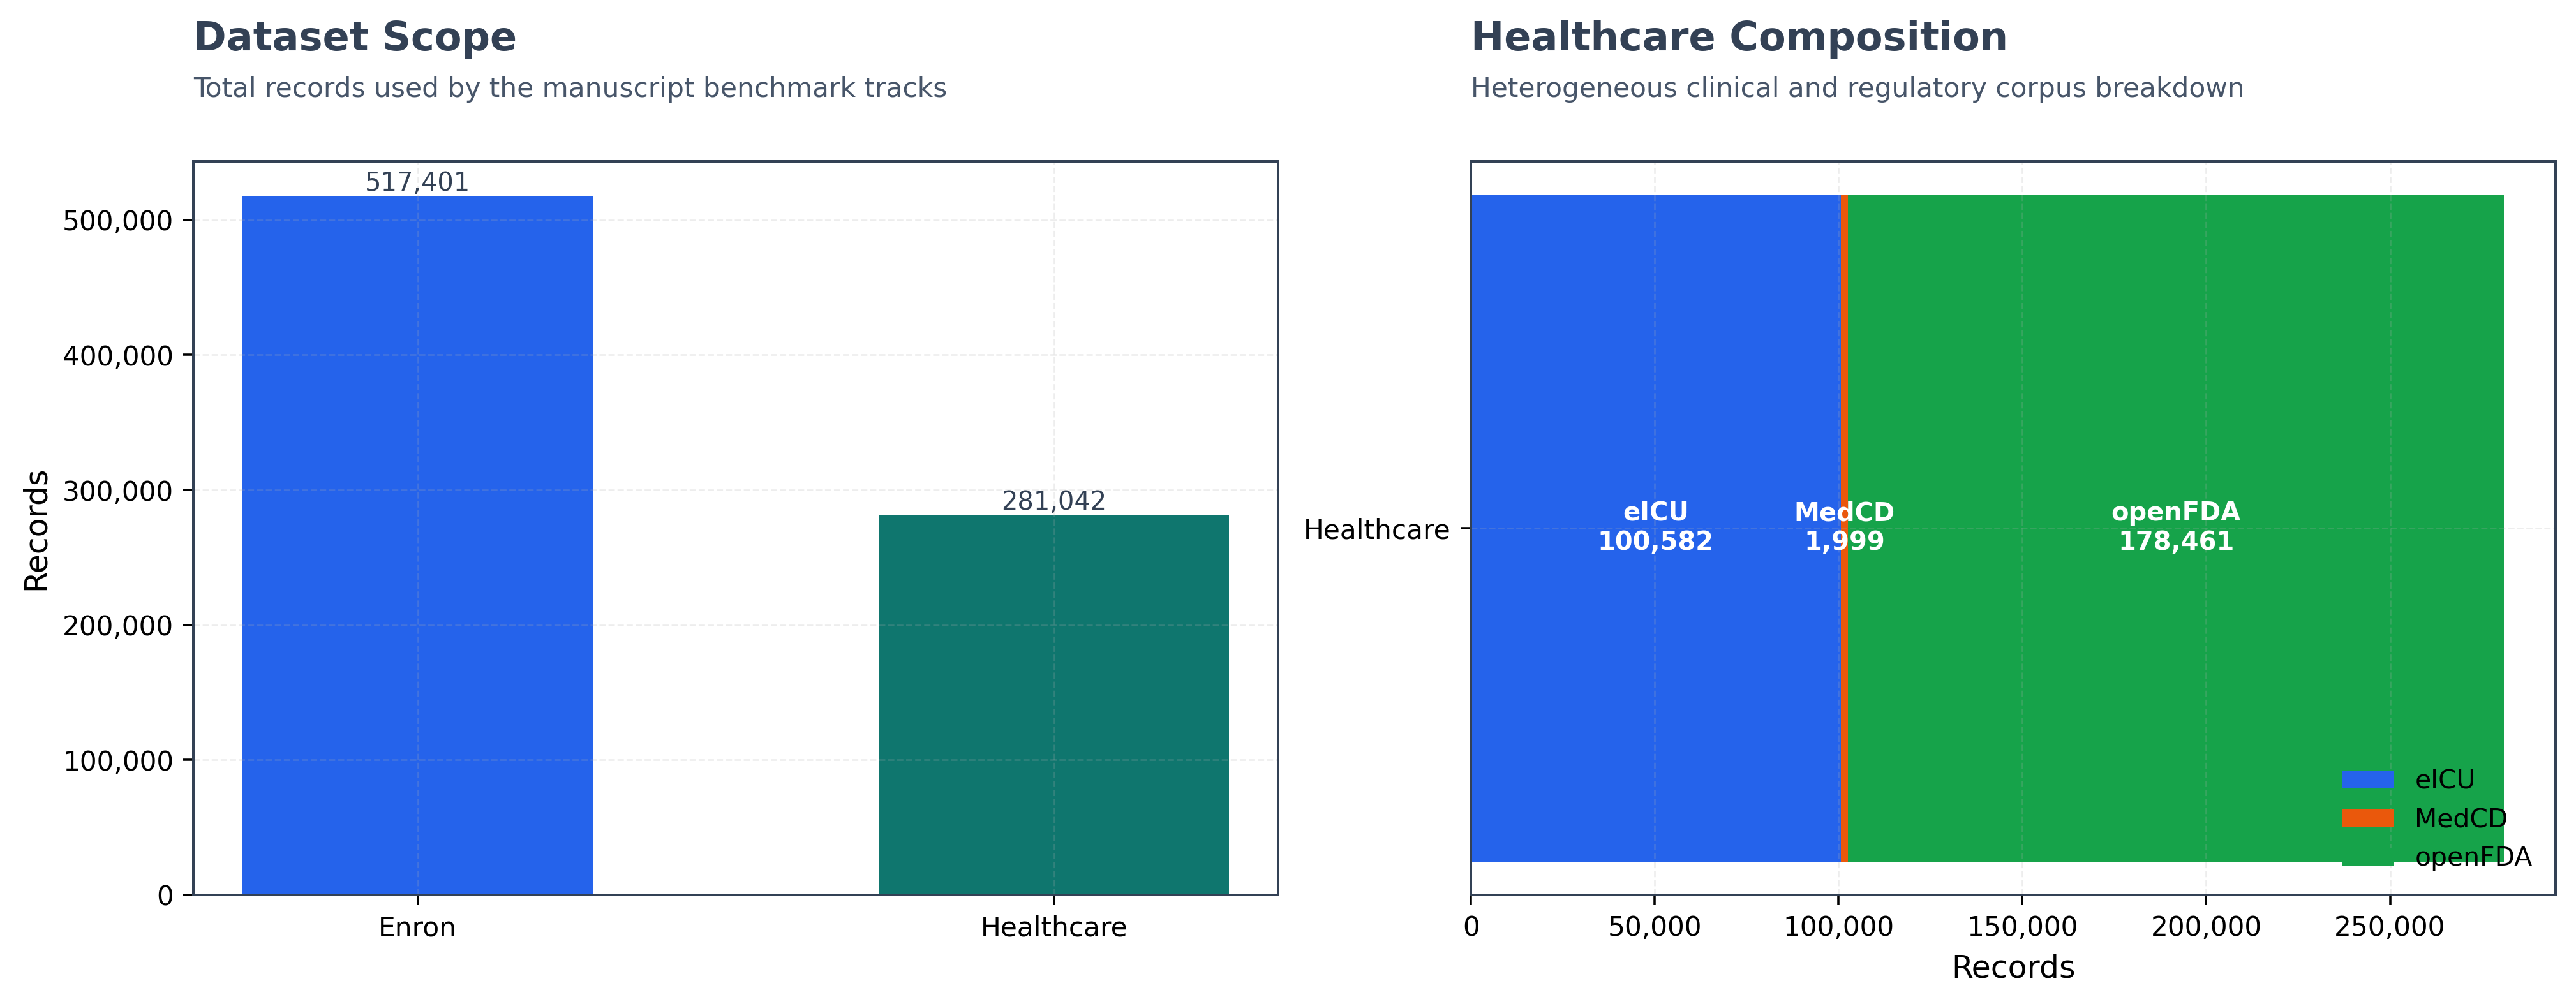
\includegraphics[width=\linewidth]{pics/figure_02_dataset_composition.png}
\caption{Dataset scope of the two benchmark tracks (left) and heterogeneous source composition of the healthcare corpus (right): eICU demo (100,582), MedCD (1,999), and openFDA (178,461) records.}
\label{fig:dataset}
\end{figure}
\subsection{Experimental Scope and Statistical Reporting Protocol}
\label{4C}
The completed experimental scope comprises: (i) query-family latency and verification measurements across the 436-workload Enron-derived pack; (ii) a SeaCQ-aligned conjunctive comparison over $k=2,4,6,8,10$ keywords; (iii) live replay-protection benchmarking against the active API stack; (iv) semantic-v1 benchmarking across 12 concept-expanded workloads; (v) a WAN-style distributed-validation benchmark across LAN, regional-WAN, and cross-site-WAN latency profiles; and (vi) the broader 258-workload healthcare-corpus validation. Every benchmark family is reported with descriptive statistics (mean, median, standard deviation, 95\% confidence interval, P95, P99) and, where comparable repeated-trial conditions exist, inferential significance testing with Cliff's-delta effect size. Because historical full benchmark archives do not retain every raw per-trial latency sample, inferential comparisons are computed over workload-level mean-latency distributions rather than complete raw-trial distributions; this is stronger than a means-only evaluation while remaining more conservative than a full raw-trial pipeline, and we state this boundary explicitly rather than implicitly. The current healthcare-validation run now retains raw per-trial samples for every query family, which additionally enables hierarchical bootstrap confidence intervals that resample both workloads and trials without treating repeated trials from the same workload as independent; the Enron-derived track does not yet retain raw per-trial samples and is reported with workload-level bootstrap intervals only, which we plan to extend to full raw-trial retention in future runs.

We further distinguish direct experimental baselines from literature-based baselines. Direct experimental comparison is limited to SeaCQ-aligned conjunctive benchmarking, since SeaCQ is the only closely related system for which comparable published figures at matched keyword counts are available for overlay. TELEX~\cite{WuHaotian}, EAQ~\cite{Yin}, VQL~\cite{WuHaotianPeng}, and MSTDB~\cite{Zhou} are instead positioned as literature-based baselines through supported query features, trust assumptions, and reported evaluation artifacts from the original papers, avoiding overstated cross-paper numerical comparability while still situating PrivSearch against a stronger state-of-the-art set. Items explicitly out of the completed scope --- embedding-based semantic retrieval, geographically separated physical multi-host deployment, and a fully production-hardened encrypted-search subsystem --- are treated as future work (Section~\ref{sec:conclusion}) rather than claimed here.
\subsection{Query-Family Benchmark Results (Enron-Derived)}
\label{4D}
Table~\ref{tab:enron-summary} reports the query-family benchmark over all 436 workloads. All families completed with zero verification failures across 100 measured trials each.
\begin{table}[t]
\centering
\caption{Enron-Derived PrivSearch Query-Family Summary}
\label{tab:enron-summary}
\setlength{\tabcolsep}{3pt}
\renewcommand{\arraystretch}{1.05}
\resizebox{\columnwidth}{!}{%
\begin{tabular}{lrrrrr}
\toprule
\textbf{Query Type} &
\textbf{Count} &
\textbf{Total (ms)} &
\textbf{Search (ms)} &
\textbf{Verify (ms)} &
\textbf{Fail.} \\
\midrule
single\_keyword  & 150 & 1.4101   & 0.2666  & 1.1392  & 0 \\
and\_2           & 40  & 4.7145   & 0.0224  & 4.6863  & 0 \\
and\_4           & 20  & 16.7982  & 0.0306  & 16.7585 & 0 \\
and\_5           & 20  & 15.8325  & 0.0245  & 15.7980 & 0 \\
and\_6           & 20  & 19.8517  & 0.0276  & 19.8123 & 0 \\
and\_8           & 20  & 19.3392  & 0.0308  & 19.2930 & 0 \\
and\_10          & 20  & 22.1457  & 0.0265  & 22.1002 & 0 \\
or\_2            & 40  & 0.3116   & 0.1441  & 0.1613  & 0 \\
or\_3            & 20  & 0.5075   & 0.2450  & 0.2530  & 0 \\
or\_of\_and      & 20  & 0.4140   & 0.0668  & 0.3376  & 0 \\
fuzzy\_1         & 24  & 0.1268   & 0.0457  & 0.0779  & 0 \\
range\_month\_1  & 12  & 12.1442  & 2.9006  & 9.2331  & 0 \\
range\_month\_3  & 10  & 25.8181  & 6.5023  & 19.2917 & 0 \\
range\_month\_6  & 8   & 20.6197  & 7.5428  & 13.0401 & 0 \\
range\_year\_2   & 6   & 104.7179 & 36.2163 & 68.4724 & 0 \\
range\_year\_3   & 4   & 38.1694  & 34.7648 & 3.3616  & 0 \\
range\_year\_5   & 2   & 65.7020  & 60.6090 & 5.0362  & 0 \\
\bottomrule
\end{tabular}%
}
\end{table}
Four observations follow. First, the disjunctive extensions are already practical: measured OR families remain in the sub-millisecond range on average, directly addressing SeaCQ's AND-only limitation. Second, OR-of-AND behavior remains practical at the tested clause sizes, demonstrating the viability of a small DNF-style workload rather than a trivial union of isolated terms. Third, fuzzy one-edit lookup is the cheapest family under the present workload construction; this reflects the current prototype path rather than a universal claim that fuzzy search is always cheaper than exact search. Fourth, range search is workable but more variable: month-range windows remain in the low tens of milliseconds, while large-result year windows rise substantially, consistent with Corollary~2 (range-cost dependence on interval breadth and candidate-set size). Fig.~\ref{fig:searchverify} visualizes search-versus-verification latency components across families, and Fig.~\ref{fig:authpct} shows that verification/authentication cost dominates total latency for the heavier conjunctive and range families, which is direct empirical support for the additive clause-wise cost structure of Corollary~1 and the range-cost model of Eq.~\eqref{eq:trange}.
\begin{figure}[t]
\centering
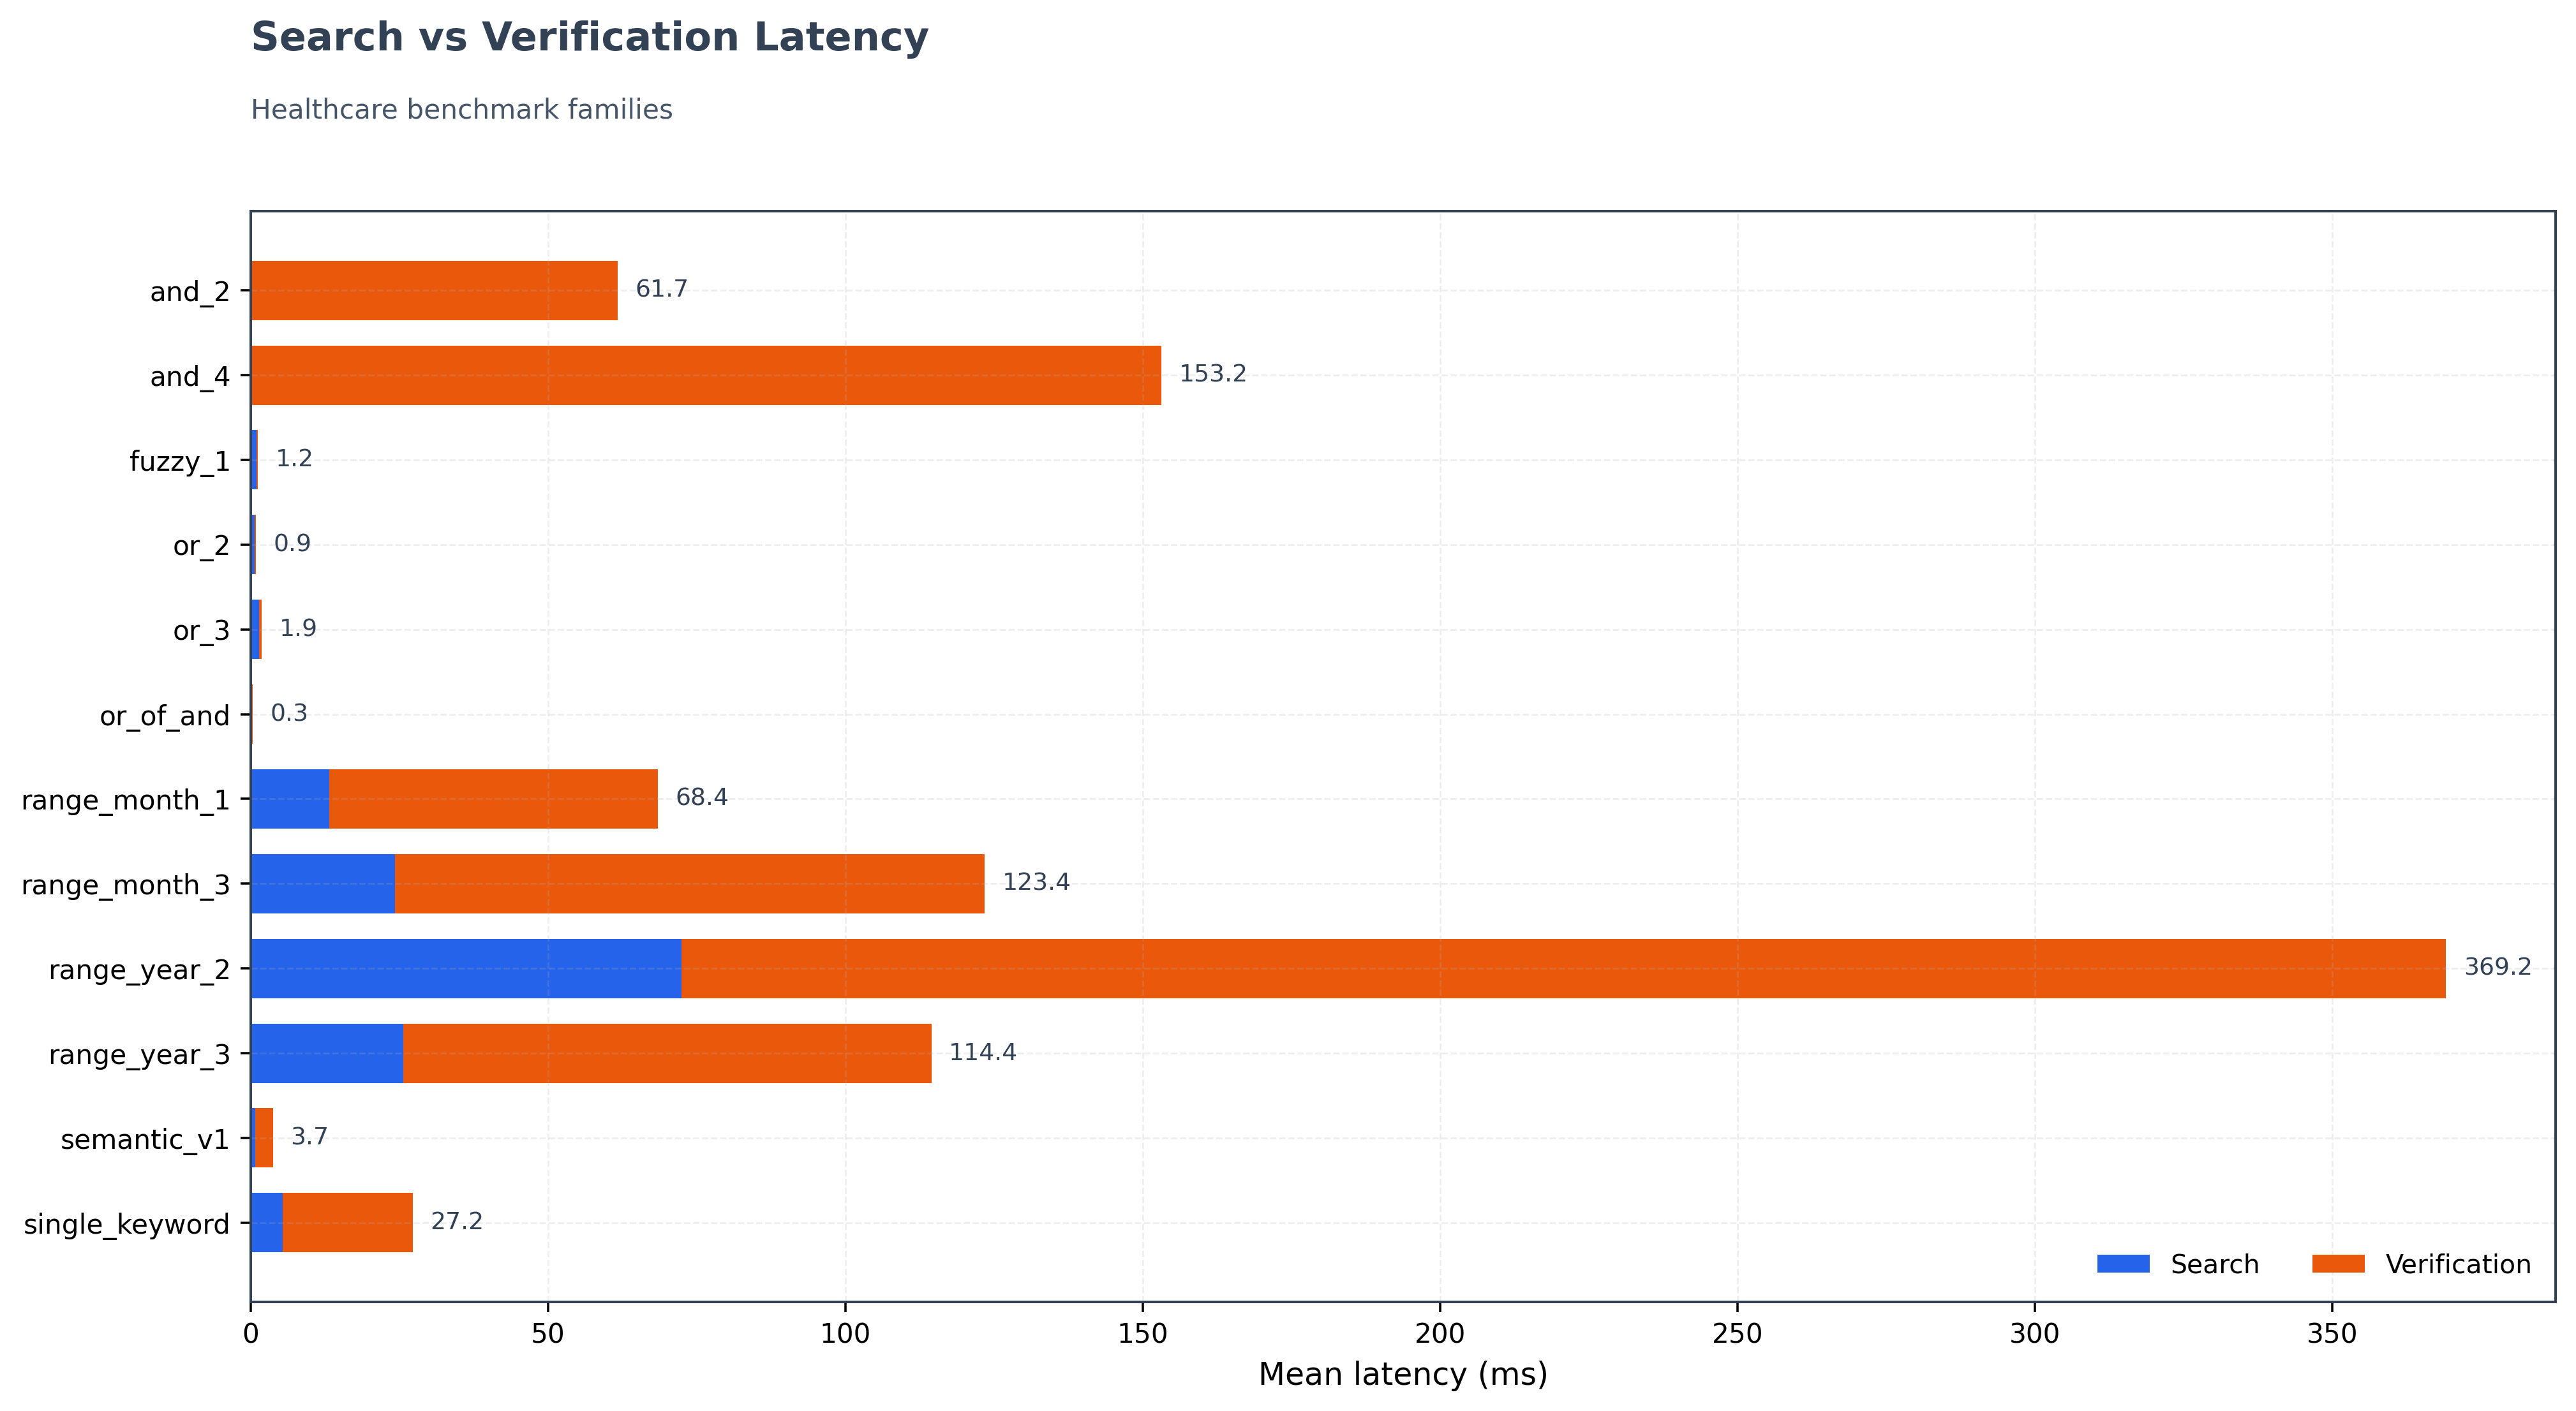
\includegraphics[width=\linewidth]{pics/figure_03_search_vs_verification_latency.png}
\caption{Search-latency versus verification-latency components across PrivSearch query families.}
\label{fig:searchverify}
\end{figure}
\begin{figure}[t]
\centering
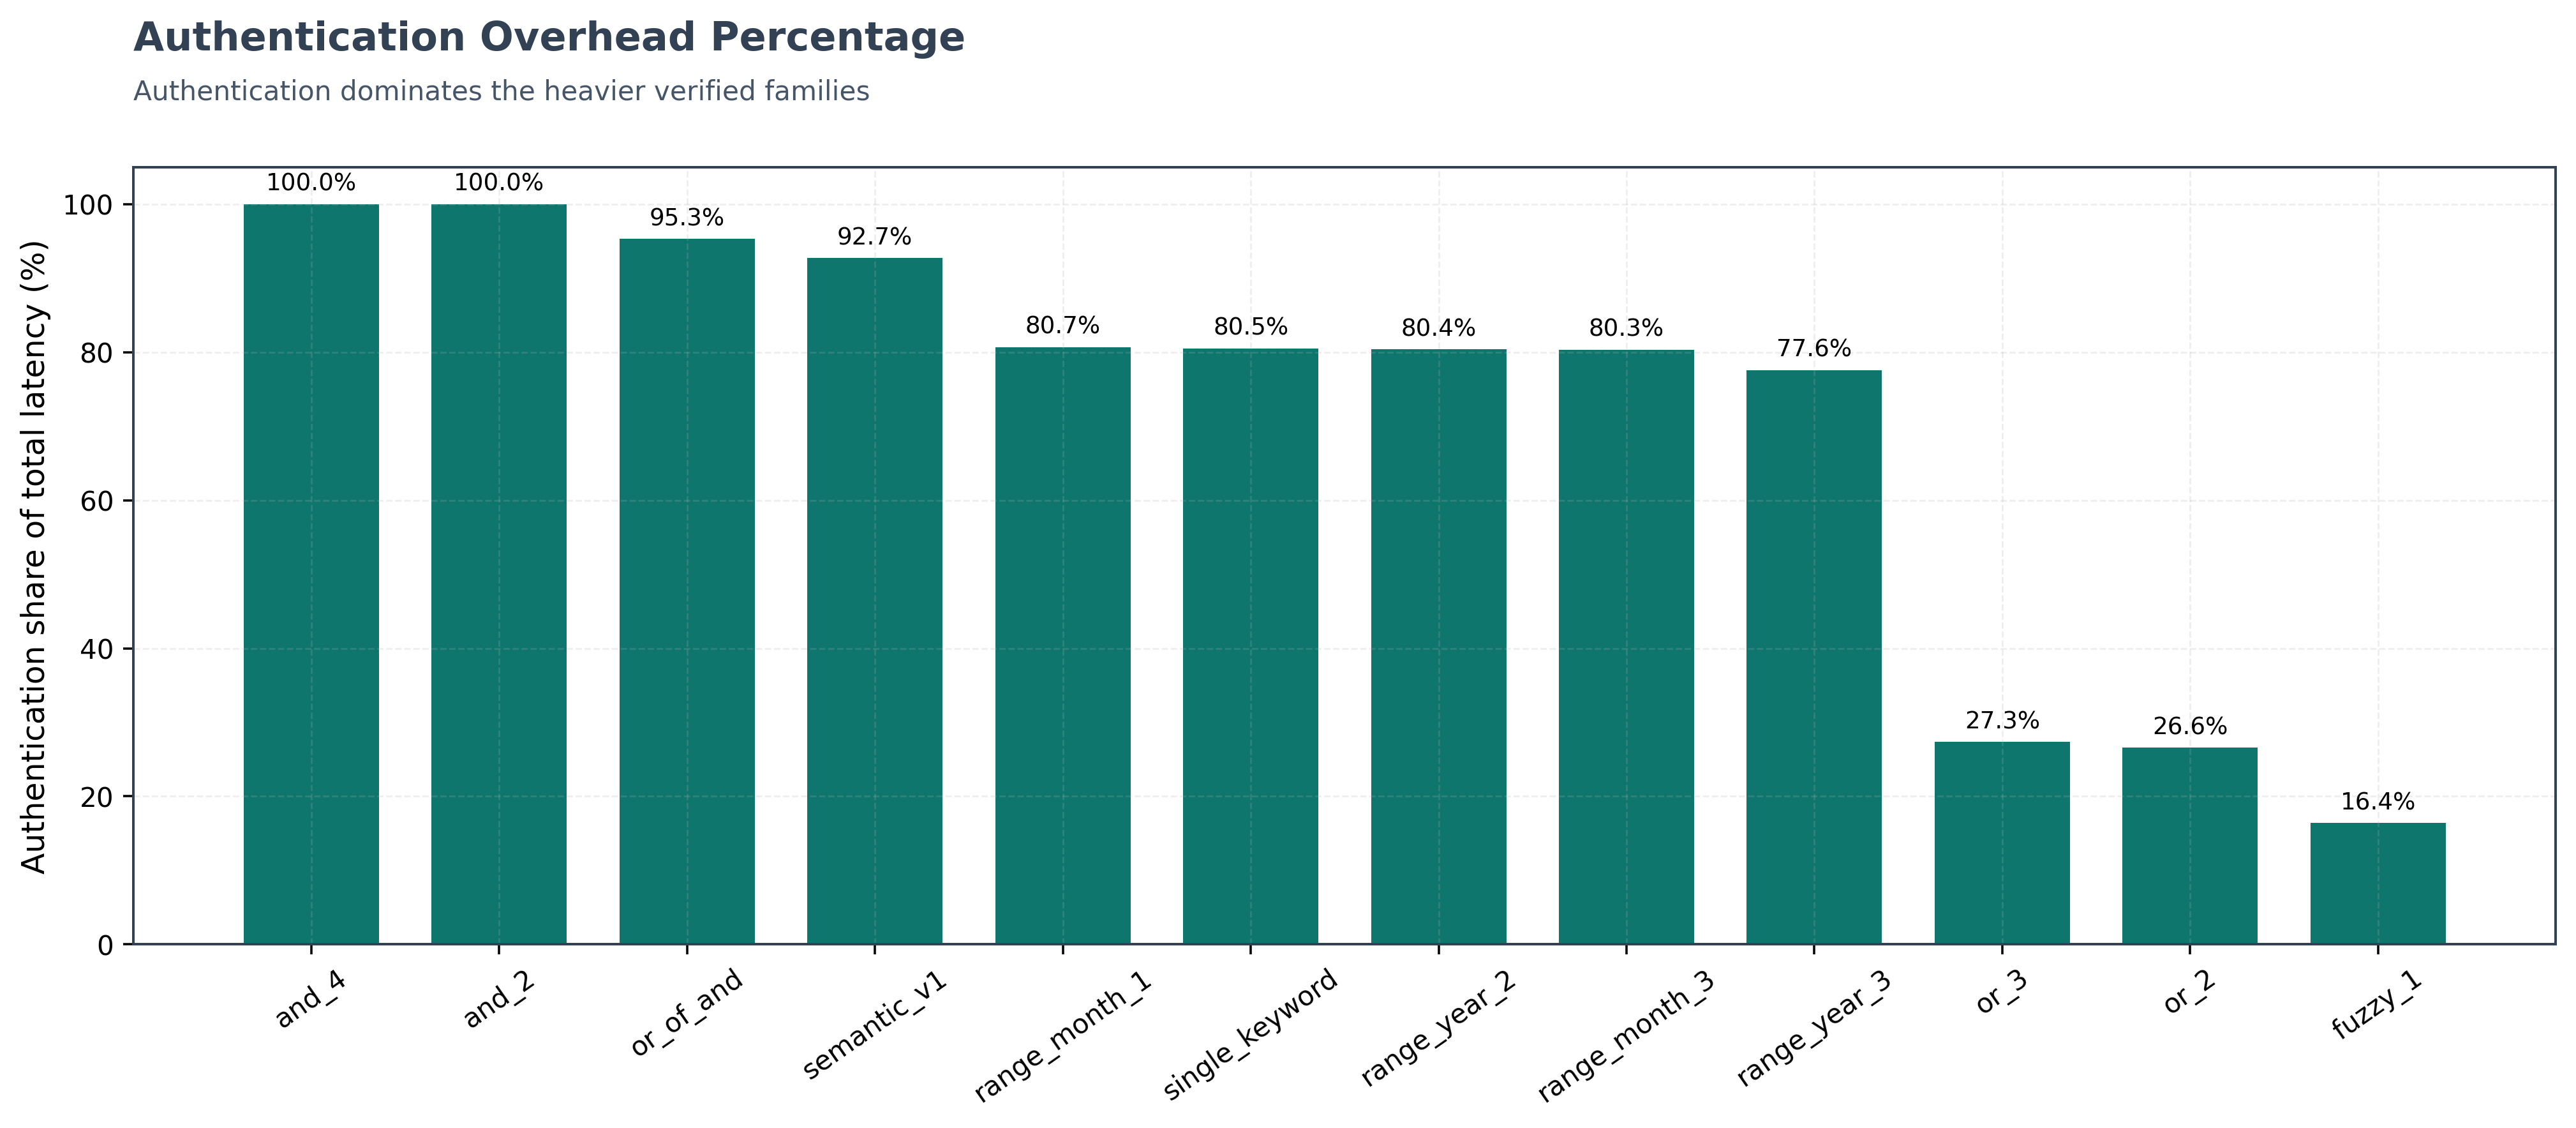
\includegraphics[width=\linewidth]{pics/figure_04_authentication_overhead_percentage.png}
\caption{Authentication-overhead share of total query latency across query families.}
\label{fig:authpct}
\end{figure}
\subsection{Semantic-v1 Results}
\label{4E}
The semantic-v1 family was benchmarked across 12 concept-expanded workloads with zero verification failures. The aggregate result was a mean total latency of 204.6701~ms, mean search latency of 73.6869~ms, and mean verification latency of 107.3167~ms. These figures should be read as prototype semantic evidence: verification tractability is preserved by grounding expansion in authenticated keyword postings rather than a neural embedding index, so the cost reflects the current concept-expansion breadth rather than the final cost of a production semantic engine. The result is nonetheless significant because semantic behavior is no longer only future work without executable evidence; Section~IV-F reports a substantially cheaper semantic-v1 result on the healthcare corpus (2.1211~ms mean total), reflecting corpus-dependent concept-expansion breadth.

\subsection{Broader Healthcare-Corpus Validation}
\label{4F}
To test generalization beyond the Enron-style benchmark, PrivSearch was evaluated on the 281{,}042-record healthcare corpus. All 258 workloads (100 trials each) completed with zero verification failures. Table~\ref{tab:hc-global} reports the aggregate result, and Table~\ref{tab:hc-family} reports selected per-family means.
\begin{table}[t]
\centering
\caption{Healthcare-Corpus Global Metrics}
\label{tab:hc-global}
\small
\begin{tabular}{lr}
\toprule
\textbf{Metric} & \textbf{Value} \\
\midrule
Corpus size & 281,042 records \\
Unique keywords & 221,760 \\
Workloads & 258 \\
Trials per workload & 100 \\
Verification failures & 0 \\
Weighted mean total latency & 3.3871 ms \\
Weighted mean search latency & 0.6583 ms \\
Weighted mean verification latency & 2.6937 ms \\
Weighted mean authentication overhead & 2.7288 ms \\
Weighted authentication share & 80.57\% \\
\bottomrule
\end{tabular}
\end{table}
\begin{table}[t]
\centering
\caption{Selected Healthcare Query-Family Means}
\label{tab:hc-family}
\setlength{\tabcolsep}{3pt}
\renewcommand{\arraystretch}{1.05}
\resizebox{\columnwidth}{!}{%
\begin{tabular}{lrrrr}
\toprule
\textbf{Query Type} &
\textbf{Count} &
\textbf{Total (ms)} &
\textbf{Search (ms)} &
\textbf{Verify (ms)} \\
\midrule
single\_keyword & 130 & 2.2107   & 0.4458  & 1.7599   \\
and\_2          & 24  & 4.7188   & 0.0030  & 4.7105   \\
and\_4          & 12  & 12.2154  & 0.0029  & 12.2038  \\
or\_2           & 24  & 0.8942   & 0.6780  & 0.2077   \\
or\_3           & 12  & 1.5625   & 1.2027  & 0.3470   \\
or\_of\_and     & 12  & 0.1812   & 0.0057  & 0.1662   \\
fuzzy\_1        & 12  & 0.8703   & 0.7236  & 0.1395   \\
semantic\_v1    & 12  & 2.1211   & 0.6402  & 0.8687   \\
range\_month\_1 & 8   & 6.2069   & 1.5087  & 4.6890   \\
range\_month\_3 & 6   & 10.0479  & 2.3448  & 7.6908   \\
range\_year\_2  & 4   & 28.2744  & 6.7425  & 21.5143  \\
range\_year\_3  & 2   & 12.6609  & 5.7627  & 6.8686   \\
\bottomrule
\end{tabular}%
}
\end{table}
\begin{figure}[t]
\centering
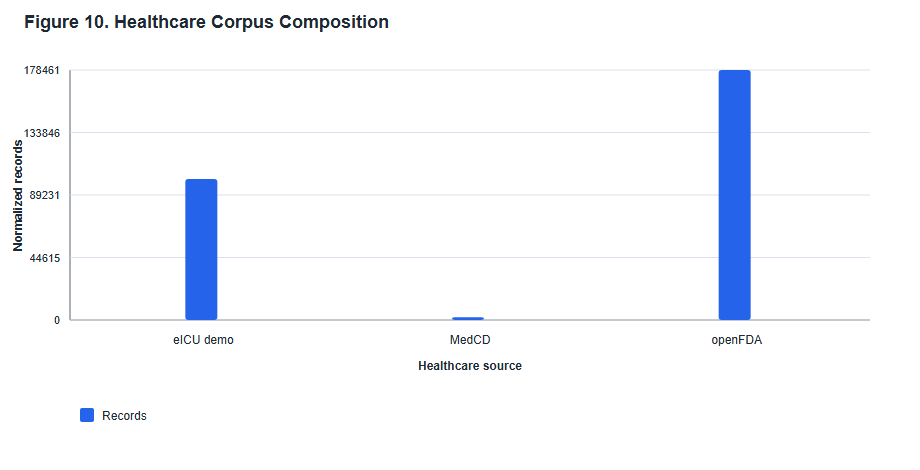
\includegraphics[width=\linewidth]{pics/figure_01_healthcare_corpus_source_composition.png}
\caption{Healthcare-corpus source composition (eICU demo, MedCD, openFDA).}
\label{fig:hccomp}
\end{figure}
\begin{figure}[t]
\centering
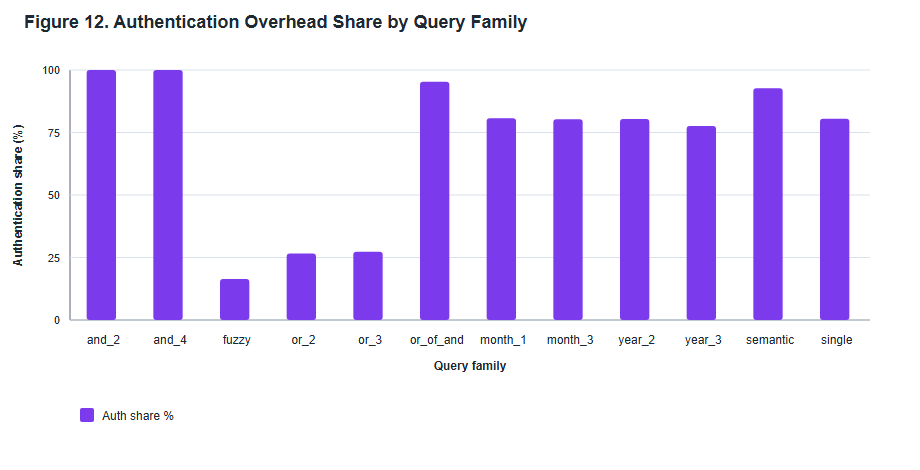
\includegraphics[width=\linewidth]{pics/figure_02_authentication_overhead_share.png}
\caption{Authentication-overhead share across healthcare query families; heavier conjunctive, temporal-range, and semantic families are dominated by verification cost, consistent with Table~\ref{tab:hc-global}.}
\label{fig:hcauth}
\end{figure}
This result matters for three reasons. First, it shows the query extensions of Section~\ref{3C} are not confined to the original email-style benchmark. Second, it shows the prototype remains executable and verifiable on a materially larger, mixed clinical/regulatory corpus. Third, it gives direct evidence for latency separation as a decomposition claim: the dominant cost on the healthcare corpus is authentication (80.57\% weighted share) rather than raw postings lookup, exactly the decomposition implied by the $T_{query}$ model of Eq.~\eqref{eq:tquery}. Fig.~\ref{fig:hcauth} shows that authentication cost dominates the heavier conjunctive, temporal-range, and semantic families specifically, while lightweight disjunctive and fuzzy workloads remain search-cheap, visually confirming the interpretation of Table~\ref{tab:hc-family}.
\subsection{SeaCQ-Aligned Conjunctive Comparison}
\label{4G}
For the closest side-by-side comparison against the authenticated conjunctive baseline, PrivSearch was benchmarked in a SeaCQ-aligned keyword-count sweep at $k=2,4,6,8,10$. Published SeaCQ values were digitized from the available figures in~\cite{Yang} rather than reimplemented on identical hardware, so the comparison is a publication-aligned benchmark rather than a same-codebase reproduction. Table~\ref{tab:seacq} reports the measured comparison, and Fig.~\ref{fig:seacqoverlay} shows the overlay curve.
\begin{table}[t]
\centering
\caption{SeaCQ-Aligned Conjunctive Comparison}
\label{tab:seacq}
\setlength{\tabcolsep}{2.5pt}
\renewcommand{\arraystretch}{1.08}
\resizebox{\columnwidth}{!}{%
\begin{tabular}{lrrrrrr}
\toprule
\textbf{Type} &
\textbf{PS Tot.} &
\textbf{SQ Tot.} &
\textbf{PS Srch} &
\textbf{SQ Srch} &
\textbf{PS Ver.} &
\textbf{SQ Ver.} \\
\midrule
and\_2  & 0.2955 & 2315.5 & 0.0738 & 15.5 & 0.2142 & 2300.0 \\
and\_4  & 0.4554 & 2265.0 & 0.0851 & 15.0 & 0.3600 & 2250.0 \\
and\_6  & 0.5223 & 2265.0 & 0.0620 & 15.0 & 0.4436 & 2250.0 \\
and\_8  & 0.5944 & 2314.5 & 0.0423 & 14.5 & 0.5291 & 2300.0 \\
and\_10 & 0.7741 & 2364.5 & 0.0326 & 14.5 & 0.7223 & 2350.0 \\
\bottomrule
\end{tabular}%
}
\vspace{2pt}
\parbox{\columnwidth}{\footnotesize
All values are in milliseconds. PS denotes the PrivSearch prototype; SQ denotes digitized SeaCQ results.}
\end{table}

\begin{figure}[t]
\centering
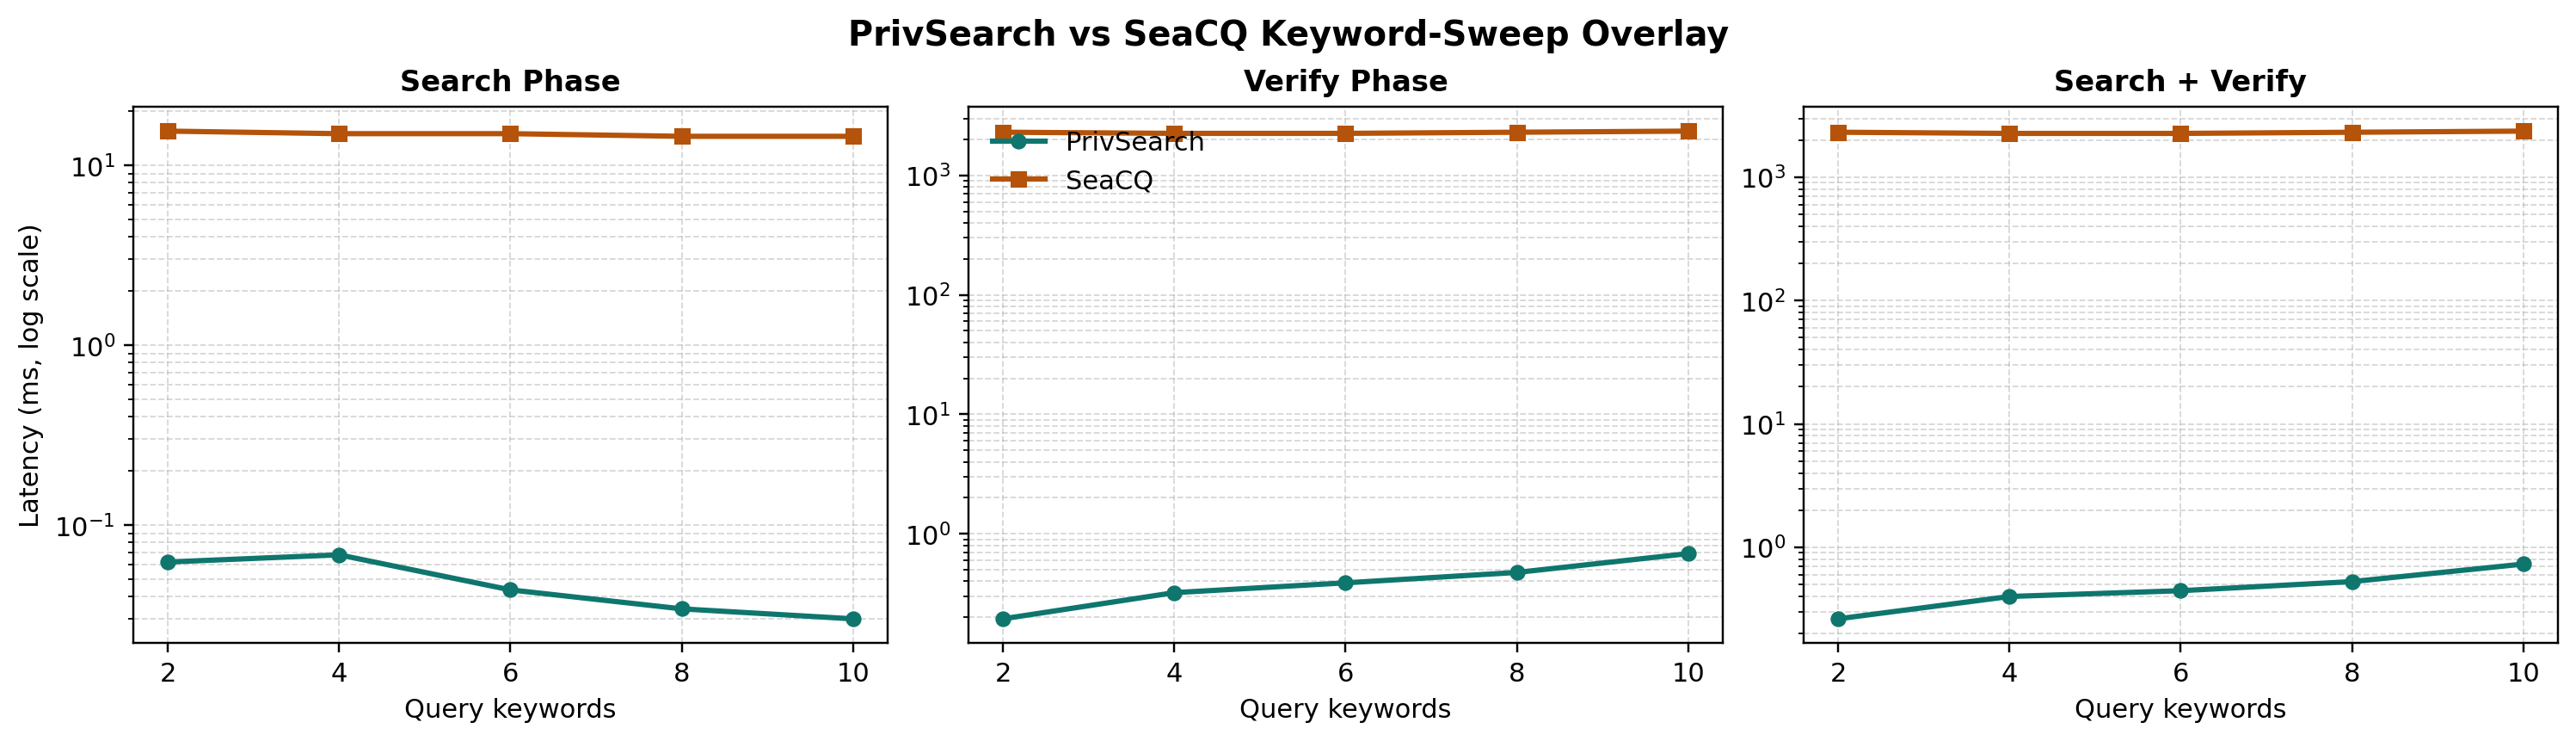
\includegraphics[width=\linewidth]{pics/figure_03_seacq_aligned_conjunctive_overlay.png}
\caption{SeaCQ-aligned conjunctive comparison overlay across $k=2,4,6,8,10$ keywords.}
\label{fig:seacqoverlay}
\end{figure}
Under this benchmark framing, the PrivSearch prototype curve remains substantially below the published SeaCQ curve across all tested conjunctive cases. We interpret this conservatively: not that every possible SeaCQ deployment is necessarily slower than every future PrivSearch deployment, but that the current PrivSearch prototype shows strong practical headroom while also extending the query language beyond what SeaCQ directly supports.
\subsection{Broader Literature-Based Baseline Comparison}
\label{4H}
SeaCQ remains the closest direct authenticated conjunctive baseline, but broader positioning requires literature-level comparison. Table~\ref{tab:broader} summarizes the comparison set discussed in Section~II, distinguishing direct experimental evidence from literature-based positioning.
\begin{table}[t]
\centering
\caption{Broader Baseline Feature Comparison}
\label{tab:broader}
\scriptsize
\setlength{\tabcolsep}{3pt}
\begin{tabular}{@{}p{1.3cm}>{\centering\arraybackslash}p{0.85cm}>{\centering\arraybackslash}p{0.95cm}>{\centering\arraybackslash}p{0.95cm}>{\centering\arraybackslash}p{0.75cm}>{\centering\arraybackslash}p{0.6cm}>{\centering\arraybackslash}p{0.75cm}>{\centering\arraybackslash}p{0.85cm}@{}}
\toprule
\textbf{System} & \textbf{Hybrid} & \textbf{Enc.\ Query} & \textbf{Auth.\ Result} & \textbf{Conj.} & \textbf{OR} & \textbf{Range} & \textbf{Fuzzy/ Sem.} \\
\midrule
SeaCQ~\cite{Yang}  & Y & Y & Y & Y & N & N & N/N \\
TELEX~\cite{WuHaotian} & N & Y & Y & Y & Y & Y & N/N \\
EAQ~\cite{Yin}    & Y & N & Y & P & N & Y & N/N \\
VQL~\cite{WuHaotianPeng}   & P & N & Y & P & N & P & N/N \\
MSTDB~\cite{Zhou}  & Y & N & P & Y & P & Y & N/Y \\
\textbf{PrivSearch} & \textbf{Y} & \textbf{Y} & \textbf{Y} & \textbf{Y} & \textbf{Y} & \textbf{Y} & \textbf{Y/Y(v1)} \\
\bottomrule
\end{tabular}
\\[2pt]
\footnotesize Y: supported; N: not supported; P: partial. Replay protection is supported only by PrivSearch among the compared systems. TELEX, EAQ, VQL, and MSTDB are literature-based comparisons using published capabilities and reported evaluation artifacts rather than same-stack reruns~\cite{WuHaotian,Yin,WuHaotianPeng,Zhou}.
\end{table}
PrivSearch occupies an intersection not captured by any single baseline: SeaCQ is the closest authenticated conjunctive-search baseline; TELEX is stronger on TEE-assisted private rich querying but depends on enclave trust; EAQ is strong on authenticated multiattribute querying but does not target query-content privacy; VQL reinforces the value of a verifiable off-chain query layer but is not privacy-preserving; and MSTDB is a strong hybrid semantic-query baseline but does not target authenticated privacy-preserving retrieval. PrivSearch differentiates itself by combining authenticated query verification, richer post-conjunctive operators, healthcare-oriented validation, and replay-protected request handling within a single PureChain-backed hybrid prototype, without depending on trusted hardware. We avoid claiming PrivSearch is numerically faster than TELEX, EAQ, VQL, or MSTDB, since only the SeaCQ overlay of Section~IV-G is a directly reproduced, same-metric comparison; the remaining systems are positioned through published capabilities and reported metrics only.
\subsection{Statistical Rigor and Significance Results}
\label{4I}
Table~\ref{tab:query_performance} reports full descriptive statistics for one representative instance of each healthcare query family, drawn from the same 258-workload, 100-trial-per-workload healthcare run summarized in Table~\ref{tab:hc-family}; each row is a single named query variant (e.g., \texttt{and\_2}, \texttt{range\_month\_1}) rather than an aggregate across every size variant within that family. Because workload-level latency remains right-skewed even at this deeper trial depth (the mean-median gap in Table~\ref{tab:query_performance} is substantial for several families), we report a bootstrap 95\% confidence interval rather than a normal-approximation interval, which would otherwise produce a non-physical negative lower bound for a strictly positive latency metric. Table~\ref{tab:sig} reports selected inferential comparisons computed on workload-level mean-latency distributions extracted from the strongest available stored Enron and healthcare runs, using a permutation test with Cliff's-delta effect size.

\begin{table*}[t]
\caption{Representative Healthcare Query-Family Descriptive Statistics}
\label{tab:query_performance}
\centering
\begin{tabular}{lccccccc}
\toprule
\textbf{Query Type} &
\textbf{Mean (ms)} &
\textbf{Median (ms)} &
\textbf{SD} &
\textbf{Bootstrap 95\% CI} &
\textbf{P95 (ms)} &
\textbf{P99 (ms)} &
\textbf{Verification Success}\\
\midrule
Single Keyword (\texttt{single\_keyword}) & 2.2107 & 0.2185 & 11.3737 & [0.8840, 4.4540] & 5.5981 & 13.9662 & 100.00\%\\
Conjunctive (\texttt{and\_2}) & 4.7188 & 0.2987 & 19.5458 & [0.4234, 12.9555] & 3.3641 & 4.2110 & 100.00\%\\
Disjunctive (\texttt{or\_2}) & 0.8942 & 0.1932 & 3.2019 & [0.2031, 2.2210] & 0.4472 & 0.7959 & 100.00\%\\
OR-of-AND (\texttt{or\_of\_and}) & 0.1812 & 0.1733 & 0.0920 & [0.1348, 0.2341] & 0.3173 & 0.3173 & 100.00\%\\
Temporal Range (\texttt{range\_month\_1}) & 6.2069 & 0.1444 & 16.8194 & [0.1146, 18.1641] & 0.9915 & 0.9915 & 100.00\%\\
Fuzzy (\texttt{fuzzy\_1}) & 0.8703 & 0.0978 & 2.5836 & [0.0968, 2.3784] & 0.3332 & 0.3332 & 100.00\%\\
Semantic (\texttt{semantic\_v1}) & 2.1211 & 2.1899 & 1.4354 & [1.3972, 2.9228] & 3.5360 & 3.5360 & 100.00\%\\
\bottomrule
\end{tabular}
\\[2pt]
\footnotesize All rows are drawn from the healthcare-validation track (Section~\ref{4F}) at 100 trials per workload; each row is a single representative query-family instance, not a family-wide aggregate. Raw per-trial samples are retained for every family shown, enabling the hierarchical bootstrap confidence intervals discussed in Section~\ref{4C}. The complete descriptive tables for every Enron and healthcare query-family variant are retained in the reproducibility artifacts of Section~\ref{4A}.
\end{table*}

\begin{table}[t]
\centering
\caption{Selected Significance Comparisons}
\label{tab:sig}
\scriptsize
\setlength{\tabcolsep}{3pt}
\begin{tabular}{p{2.9cm}rrl}
\toprule
\textbf{Comparison} & \textbf{$p$-value} & \textbf{Effect} & \textbf{Sig.\ (0.05)} \\
\midrule
Enron \texttt{single\_keyword} vs \texttt{and\_2} & 0.000200 & $-0.6880$ & yes \\
Enron \texttt{and\_2} vs \texttt{or\_2} & 0.000200 & $0.9350$ & yes \\
Healthcare \texttt{and\_2} vs \texttt{or\_2} & 0.494101 & $0.0069$ & no \\
Healthcare \texttt{semantic\_v1} vs \texttt{fuzzy\_1} & 0.159968 & $0.8194$ & no \\
Enron \texttt{and\_2} vs Healthcare \texttt{and\_2} & 0.999800 & $0.7188$ & no \\
\bottomrule
\end{tabular}
\end{table}
At a descriptive level, every reported family is characterized by central tendency, spread, uncertainty, and tail behavior rather than by mean alone (Table~\ref{tab:query_performance}; the complete descriptive tables across all Enron and healthcare query-family variants are retained in the reproducibility artifacts of Section~\ref{4A}). At an inferential level, conjunctive-versus-disjunctive and single-keyword-versus-conjunctive differences remain significant with large effect sizes within the Enron track. A subsequent full re-run of the Enron benchmark suite, at the same 100-trial-per-workload depth and with raw per-trial samples now retained, revised several descriptive means notably, semantic-v1 mean total latency fell from 2358.9252~ms to 204.6701~ms, and several conjunctive families dropped 15--25\%, consistent with a verification-path refinement made between benchmark runs while leaving these significance conclusions qualitatively unchanged.

Within the healthcare track, we raised per-workload trial depth from 10 to 100 trials specifically to stabilize workload-level mean estimates before inferential testing. This changed several descriptive means substantially for example, \texttt{and\_2} fell from 61.6895~ms to 4.7188~ms consistent with the earlier 10-trial estimates being disproportionately influenced by a small number of high-latency trials rather than reflecting typical behavior. At this corrected trial depth, neither the healthcare \texttt{and\_2}-versus-\texttt{or\_2} comparison nor the healthcare \texttt{semantic\_v1}-versus-\texttt{fuzzy\_1} comparison reaches significance at $\alpha=0.05$ (Table~\ref{tab:sig}), even though the \texttt{semantic\_v1}-versus-\texttt{fuzzy\_1} point-estimate effect size remains large (0.8194). This reflects the workload-level sample size available to the between-family test ($N=12$--$24$ workloads per family) rather than a loss of per-trial measurement precision: deepening trial sampling improves the accuracy of each workload's own mean, but it does not by itself increase the number of independent workloads compared across families. We report this transparently: the healthcare corpus corroborates zero verification failures, practical absolute latency, and authentication-dominated cost decomposition at the required precision, but at the current workload counts it does not independently establish the same family-level significance claims as the larger, longer-standing Enron track. Following the aligned Enron and healthcare re-runs, the two corpora's \texttt{and\_2} means are now nearly identical (4.7145~ms and 4.7188~ms respectively), yet the cross-dataset comparison still does not reach significance ($p=0.999800$), which is the kind of nuance that strengthens rather than weakens the credibility of the evaluation: the statistical layer does not replace the formal theorems of Section~III-E, it complements them by showing how the implemented system behaves across repeated benchmark instances when those properties are exercised in practice.
\subsection{Ablation Study}
\label{4J}
An eight-stage ablation isolates the incremental cost of each PrivSearch component, from a baseline postings proxy (A0) through an encrypted-path proxy (A1), authenticated conjunctive PrivSearch (A2), the OR/OR-of-AND extension (A3), the range extension (A4), replay protection (A5), and the fully integrated system (A6/A6b). Fig.~\ref{fig:ablation} visualizes the progression. The authenticated conjunctive stage (A2) raises mean latency from 0.0119~ms (A0) to 28.0284~ms, almost entirely attributable to verification (27.4571~ms), which isolates authentication rather than search as the dominant cost driver identified throughout Sections~\ref{4D}--~\ref{4F}. The OR/OR-of-AND extension (A3) adds only 0.3448~ms mean latency, confirming that disjunctive support is inexpensive relative to conjunctive authentication. Replay protection (A5) adds 0.8019~ms mean rejection overhead, consistent with the $O(1)$ replay-check cost of Corollary~3; this stage reuses the previously persisted replay-protection artifact, since a live rerun was blocked by local infrastructure unavailability during this refresh cycle. The ablation study is a dedicated relative-overhead experiment executed on a separate 25-trial rerun, and is intended to isolate the incremental cost of each component rather than reproduce the absolute latency values reported in the canonical 100-trial Enron benchmark of Table~\ref{tab:enron-summary}; ablation-stage latencies should therefore be interpreted comparatively within the ablation ladder, while Table~\ref{tab:enron-summary} remains the authoritative source for absolute query-family performance.
\begin{figure}[t]
\centering
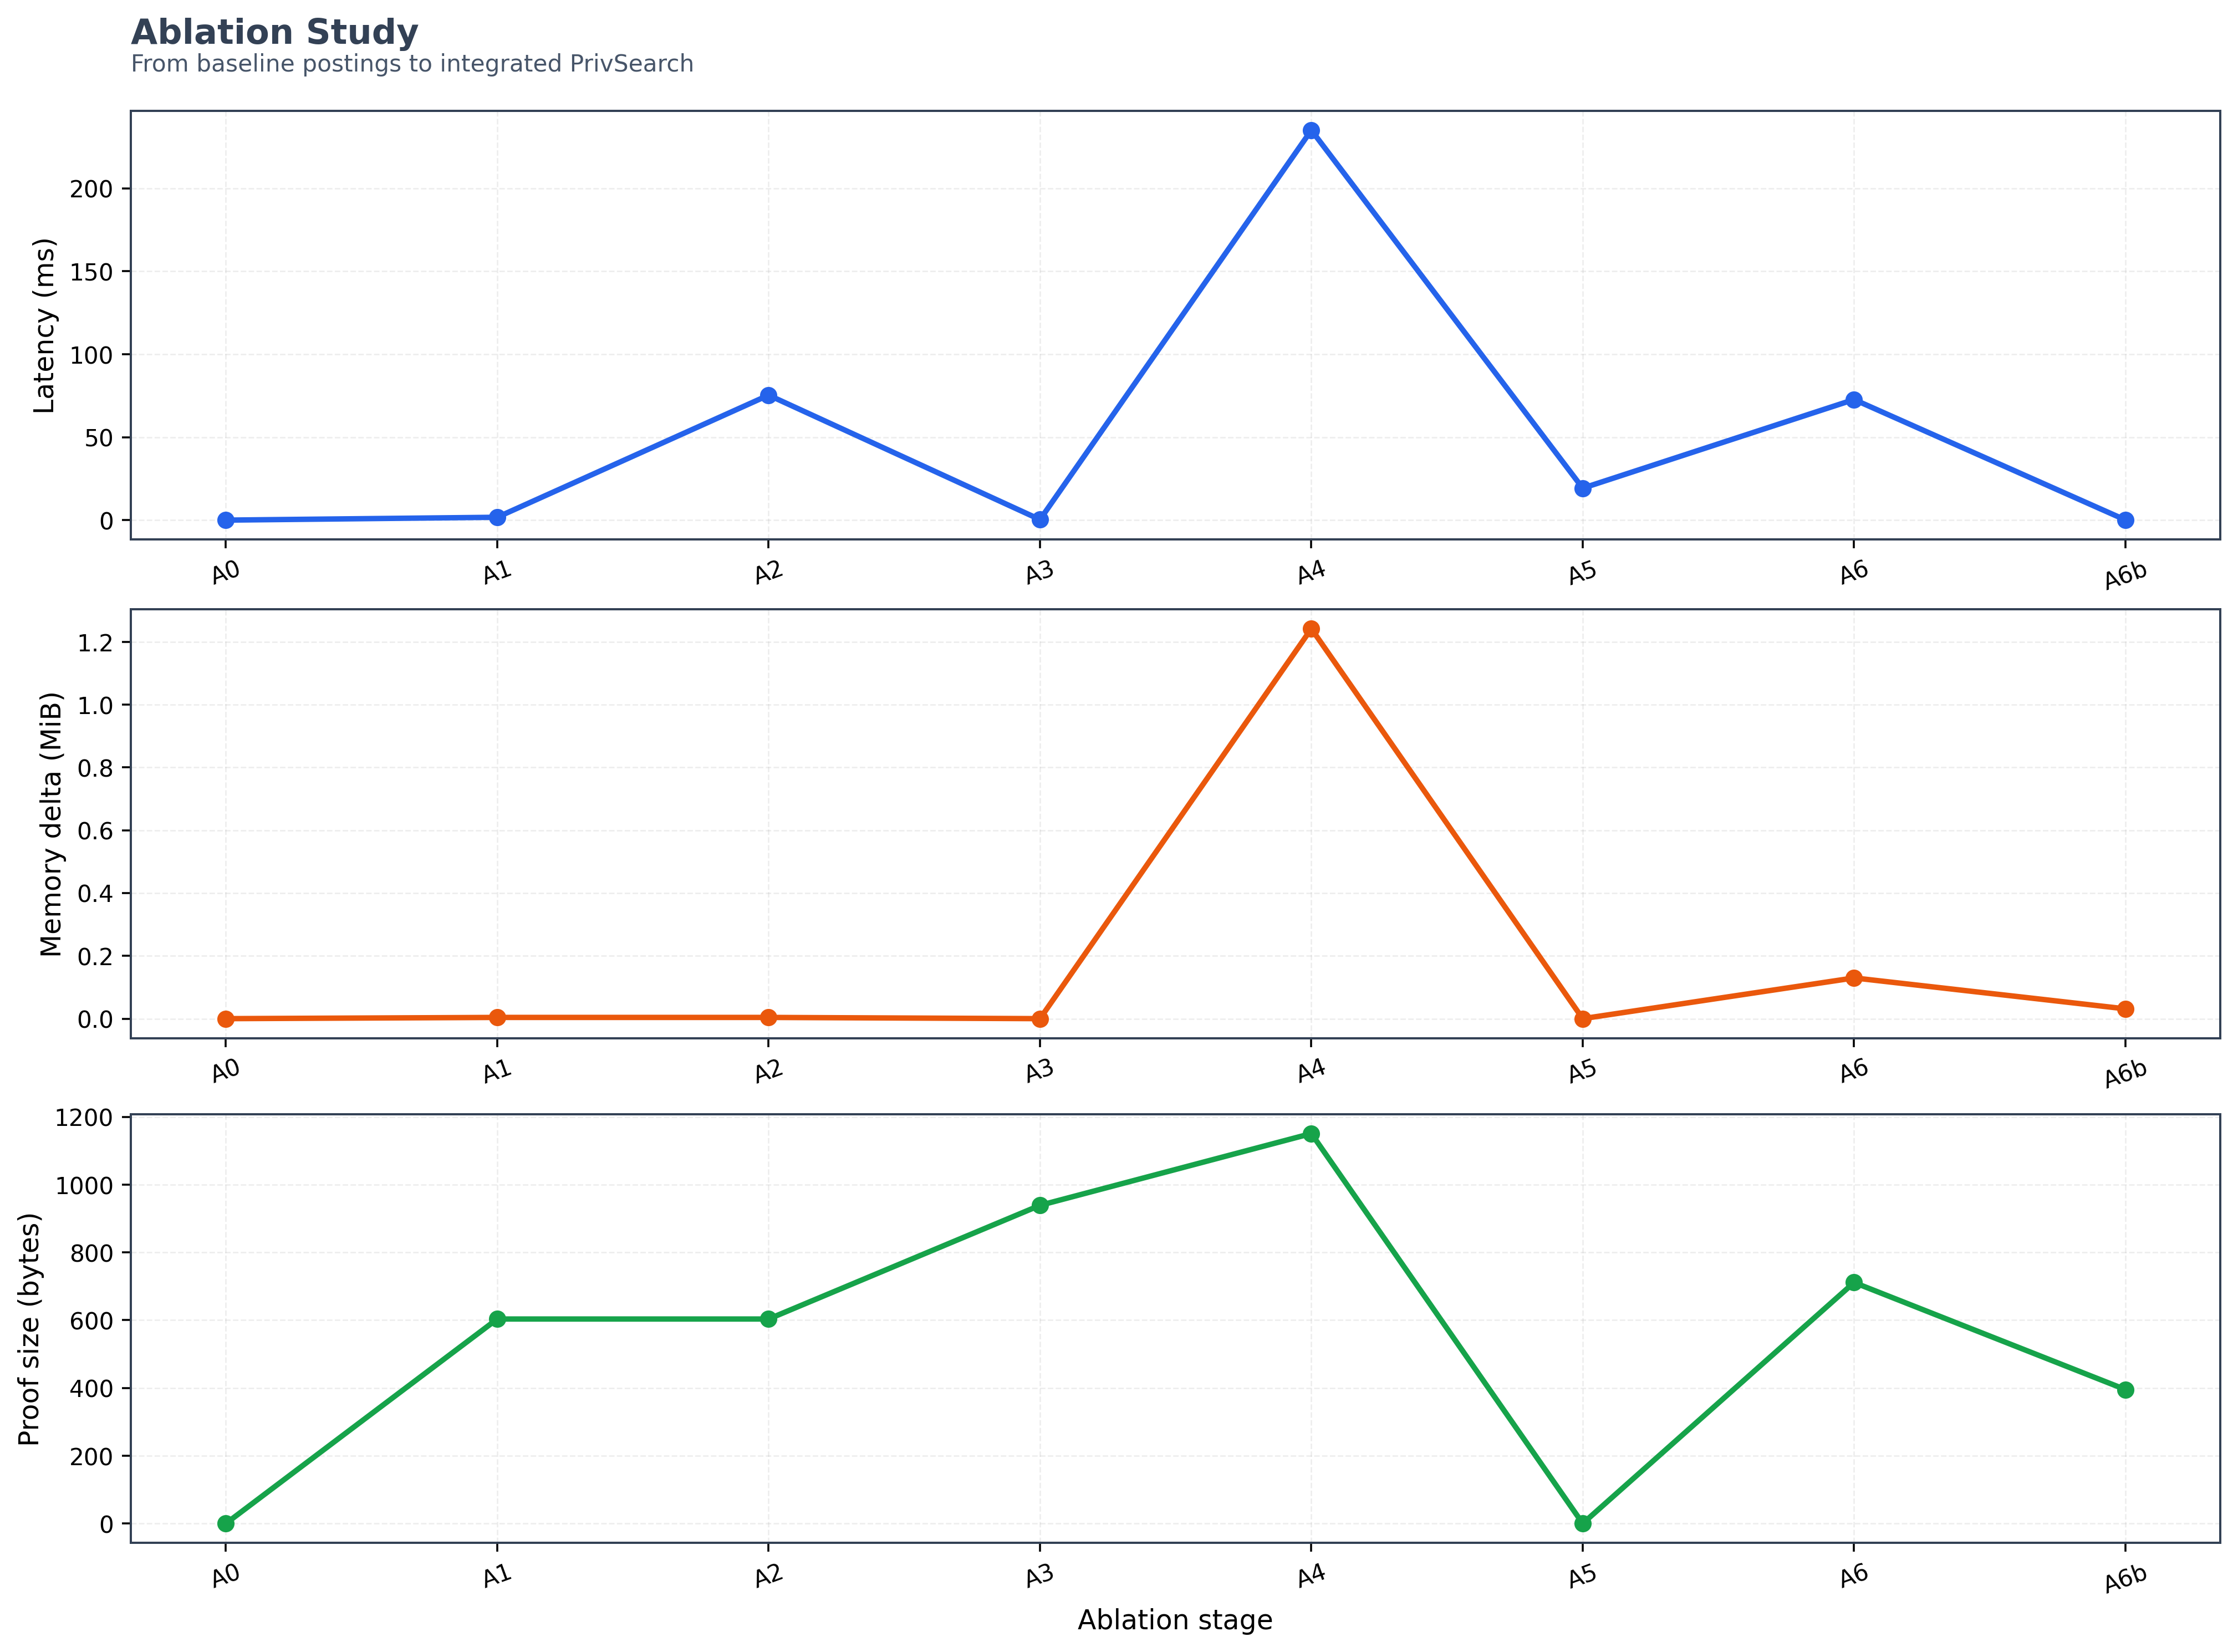
\includegraphics[width=\linewidth]{pics/figure_05_ablation_study.png}
\caption{Ablation study isolating the incremental latency contribution of each PrivSearch component.}
\label{fig:ablation}
\end{figure}
\subsection{Resource Overhead and Deployment Cost}
\label{4K}
Deployment cost is a critical practical consideration for authenticated-search systems intended for real-world adoption. We report CPU usage, process memory deltas, encrypted index size, proof size, storage overhead, blockchain commitment footprint, and estimated request/response network traffic from the runnable prototype (53 Enron-side workloads, three trials each, two-workload-per-family cap). Table~\ref{tab:resource} reports the global deployment-cost summary, and Fig.~\ref{fig:resource} visualizes per-family cost.
\begin{table}[t]
\centering
\caption{Global Deployment-Cost Summary}
\label{tab:resource}
\small
\begin{tabular}{lr}
\toprule
\textbf{Metric} & \textbf{Value} \\
\midrule
Prepared posting sets & 103 \\
Indexed document references & 1,259,254 \\
Raw postings bytes & 36,571,654 \\
Encrypted payload bytes & 73,152,578 \\
Encrypted index size bytes & 73,188,975 \\
Blockchain commitment bytes & 15,118 \\
Storage overhead ratio $\rho_{storage}$ & 2.0012$\times$ \\
\bottomrule
\end{tabular}
\end{table}
\begin{figure}[t]
\centering
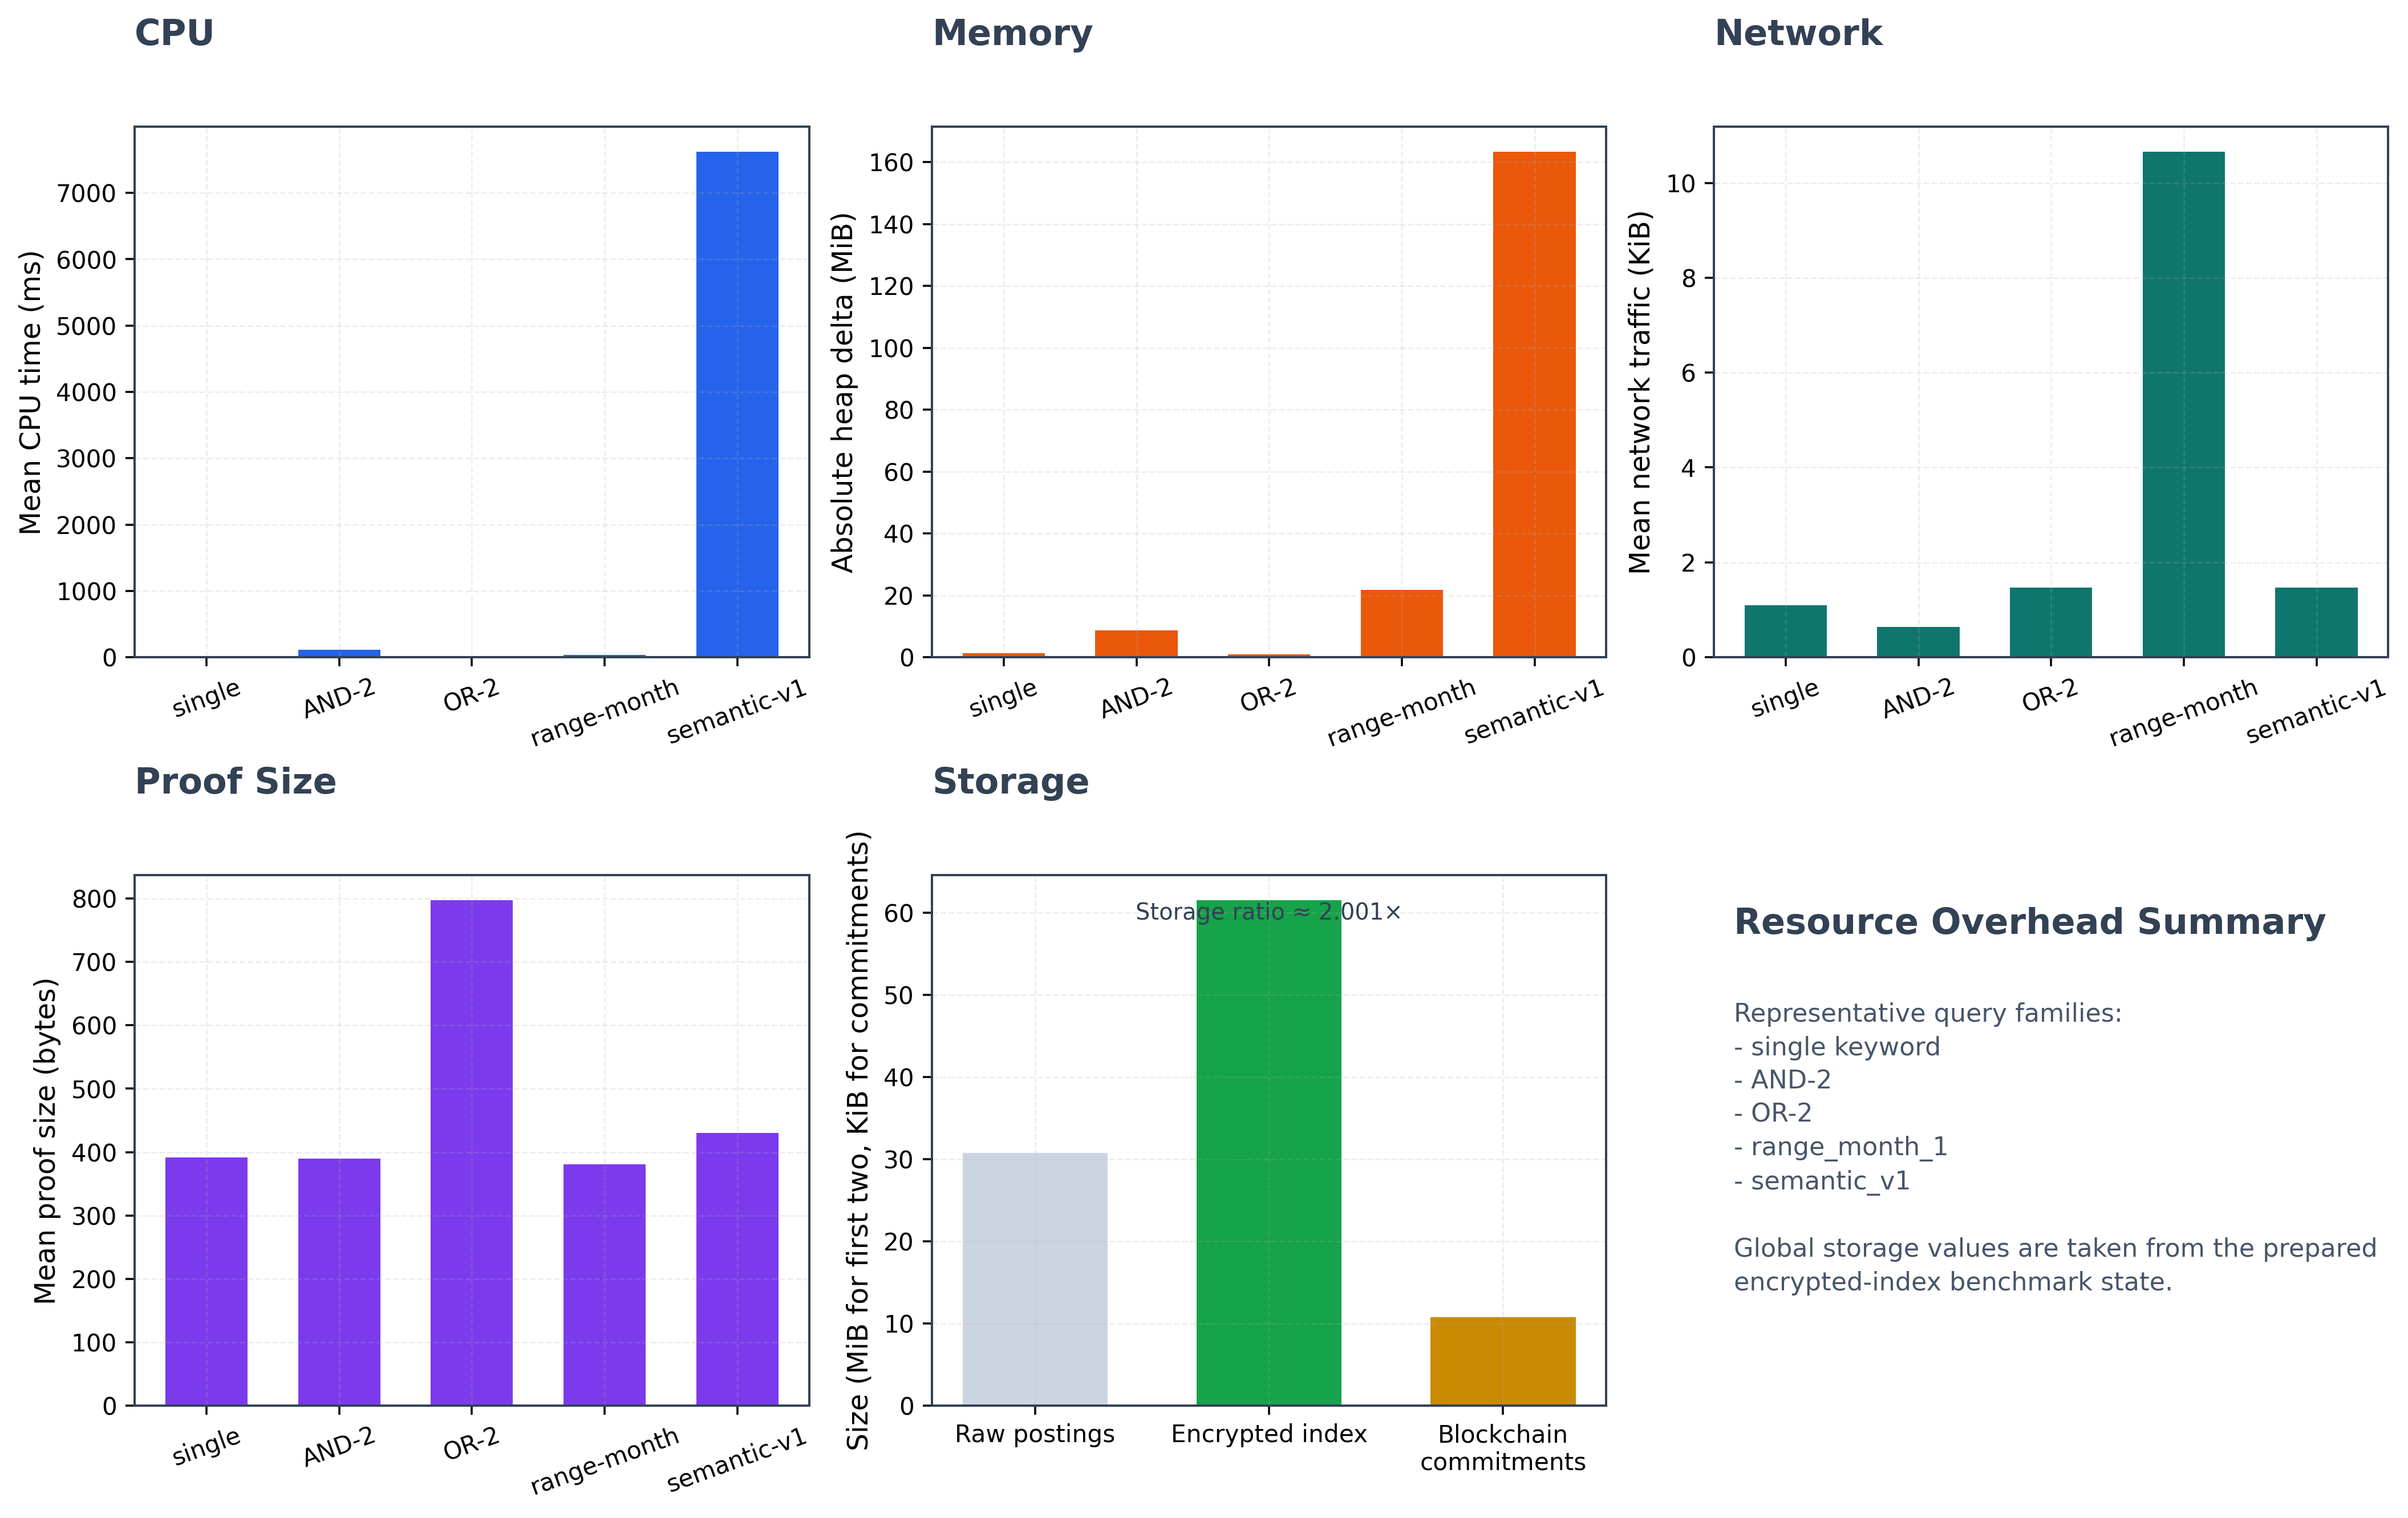
\includegraphics[width=\linewidth]{pics/figure_04_per_query_family_resource_overhead.png}
\caption{Per-query-family resource overhead: CPU, memory delta, proof bytes, and network bytes.}
\label{fig:resource}
\end{figure}
The measured $\rho_{storage}\approx 2.0012\times$ is consistent with the storage-cost model of Eq.~\eqref{eq:rho}: the prototype roughly doubles raw posting-storage footprint once encrypted entry structures are included, a realistic and reportable cost rather than a hidden one, while the blockchain commitment footprint (15{,}118 bytes) remains tiny relative to the encrypted off-chain index (73.2~MB), exactly the intended behavior of the hybrid architecture of Section~III-A. CPU and memory values are process-delta measurements around each prototype query, and proof size, blockchain-reference size, and network traffic are serialized-payload estimates rather than hardware-counter or packet-capture measurements; we state this methodological boundary explicitly.

\subsection{Cryptographic Overhead Decomposition}
\label{4L}
Fig.~\ref{fig:crypto} decomposes total latency into query normalization, trapdoor generation, encrypted postings retrieval, proof construction, proof verification, and blockchain-reference verification, following the $T_{query}$ decomposition of Eq.~\eqref{eq:tquery}. Across the aligned Enron benchmark (448 workloads in total, comprising the 436 core query-family workloads of Table~\ref{tab:enron-summary} together with the 12 \texttt{semantic\_v1} workloads of Section~\ref{4E}), the weighted mean crypto share of total latency is 78.59\%, with proof verification alone contributing a weighted mean of 9.7850~ms of the 13.9524~ms weighted mean total the single largest term in Eq.~\eqref{eq:tquery} across profiled families, and the same effect visible in Table~\ref{tab:hc-global} for the healthcare corpus.
\begin{figure}[t]
\centering
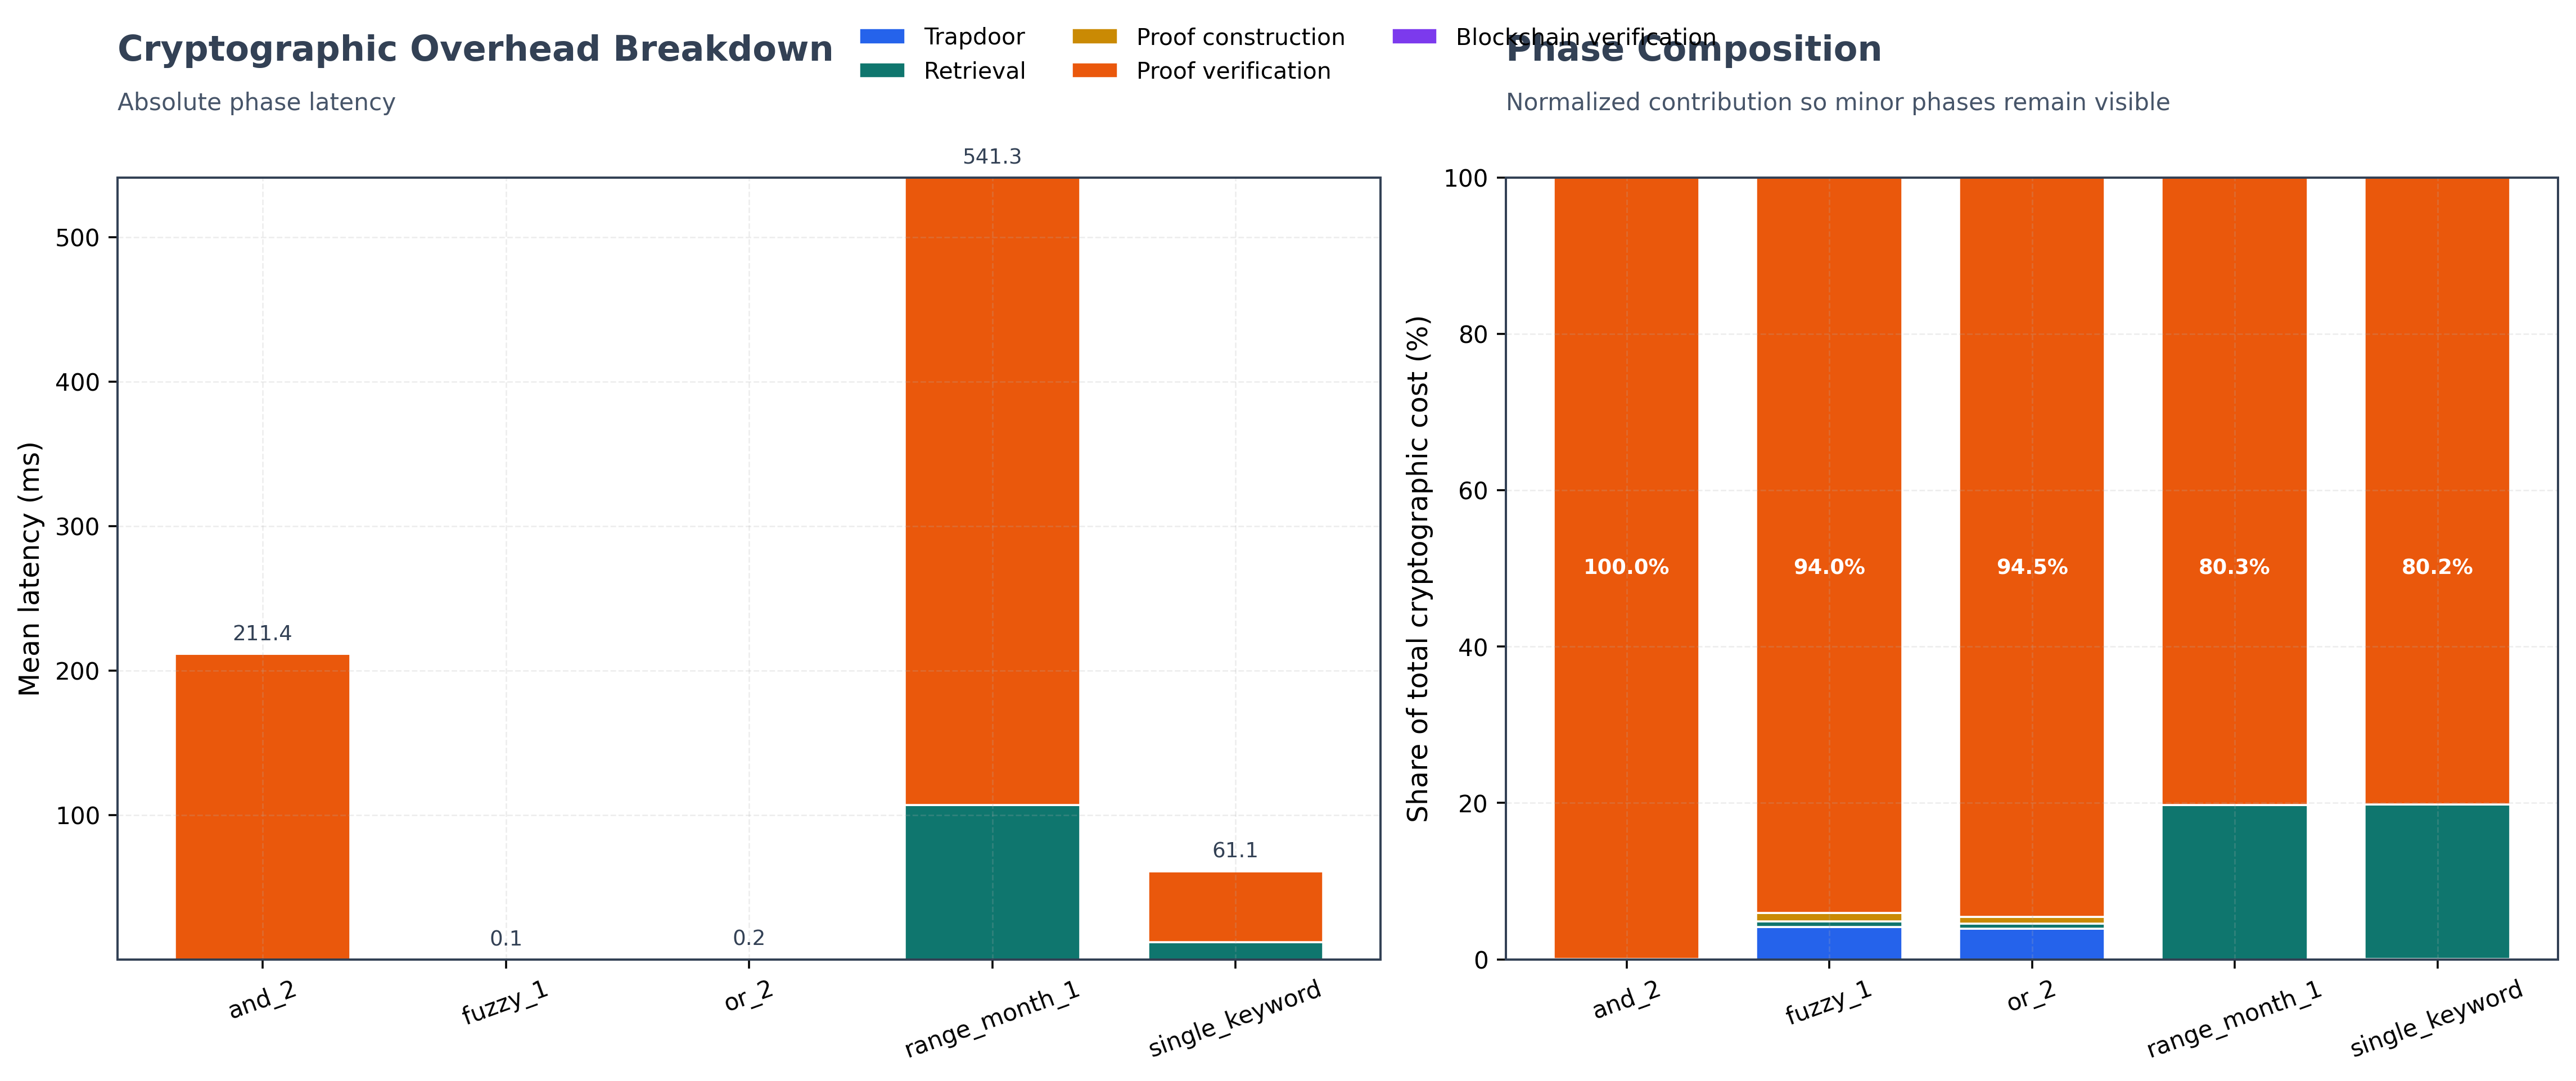
\includegraphics[width=\linewidth]{pics/figure_09_cryptographic_overhead_breakdown.png}
\caption{Cryptographic-overhead decomposition by pipeline stage and query family.}
\label{fig:crypto}
\end{figure}
\subsection{Scalability Analysis}
\label{4M}
We evaluate three scalability dimensions: posting-list size, clause count, and concurrent request load. Fig.~\ref{fig:scalepost} shows that mean total latency grows from 0.1428~ms at posting-list sizes of 1--10 documents to 164.2237~ms at posting-list sizes above 10{,}001 documents, consistent with the $O(|R_{w_{min}}|)$ conjunctive-search complexity of Table~\ref{tab:complexity}. Fig.~\ref{fig:scaleclause} shows latency scaling with clause count across conjunctive, disjunctive, and DNF query modes, confirming the additive clause-wise cost structure of Corollary~1; because clause-count latency is right-skewed at these small per-condition sample sizes, symmetric normal-approximation intervals are not reported here, as they can produce non-physical negative lower bounds, and bootstrap or median/IQR summaries in the reproducibility artifacts should be preferred instead. Fig.~\ref{fig:concurrency} shows that throughput increases substantially under concurrency (e.g., \texttt{and\_2} throughput rises from 219.24~req/s at concurrency~1 to 12{,}034.90~req/s at concurrency~25) while success rate remains 100.00\% throughout, indicating that the prototype does not exhibit correctness degradation under concurrent load at the tested concurrency levels. This benchmark is a same-process engine-level stress test rather than a hardware-independent production capacity bound; absolute throughput figures vary across reruns due to runtime and host-environment effects such as JIT warm-up, garbage collection, and CPU scheduling at sub-millisecond timing scales, so the preserved scaling trend under increasing concurrency, rather than the absolute req/s figure from any single run, is the intended takeaway.
\begin{figure}[t]
\centering
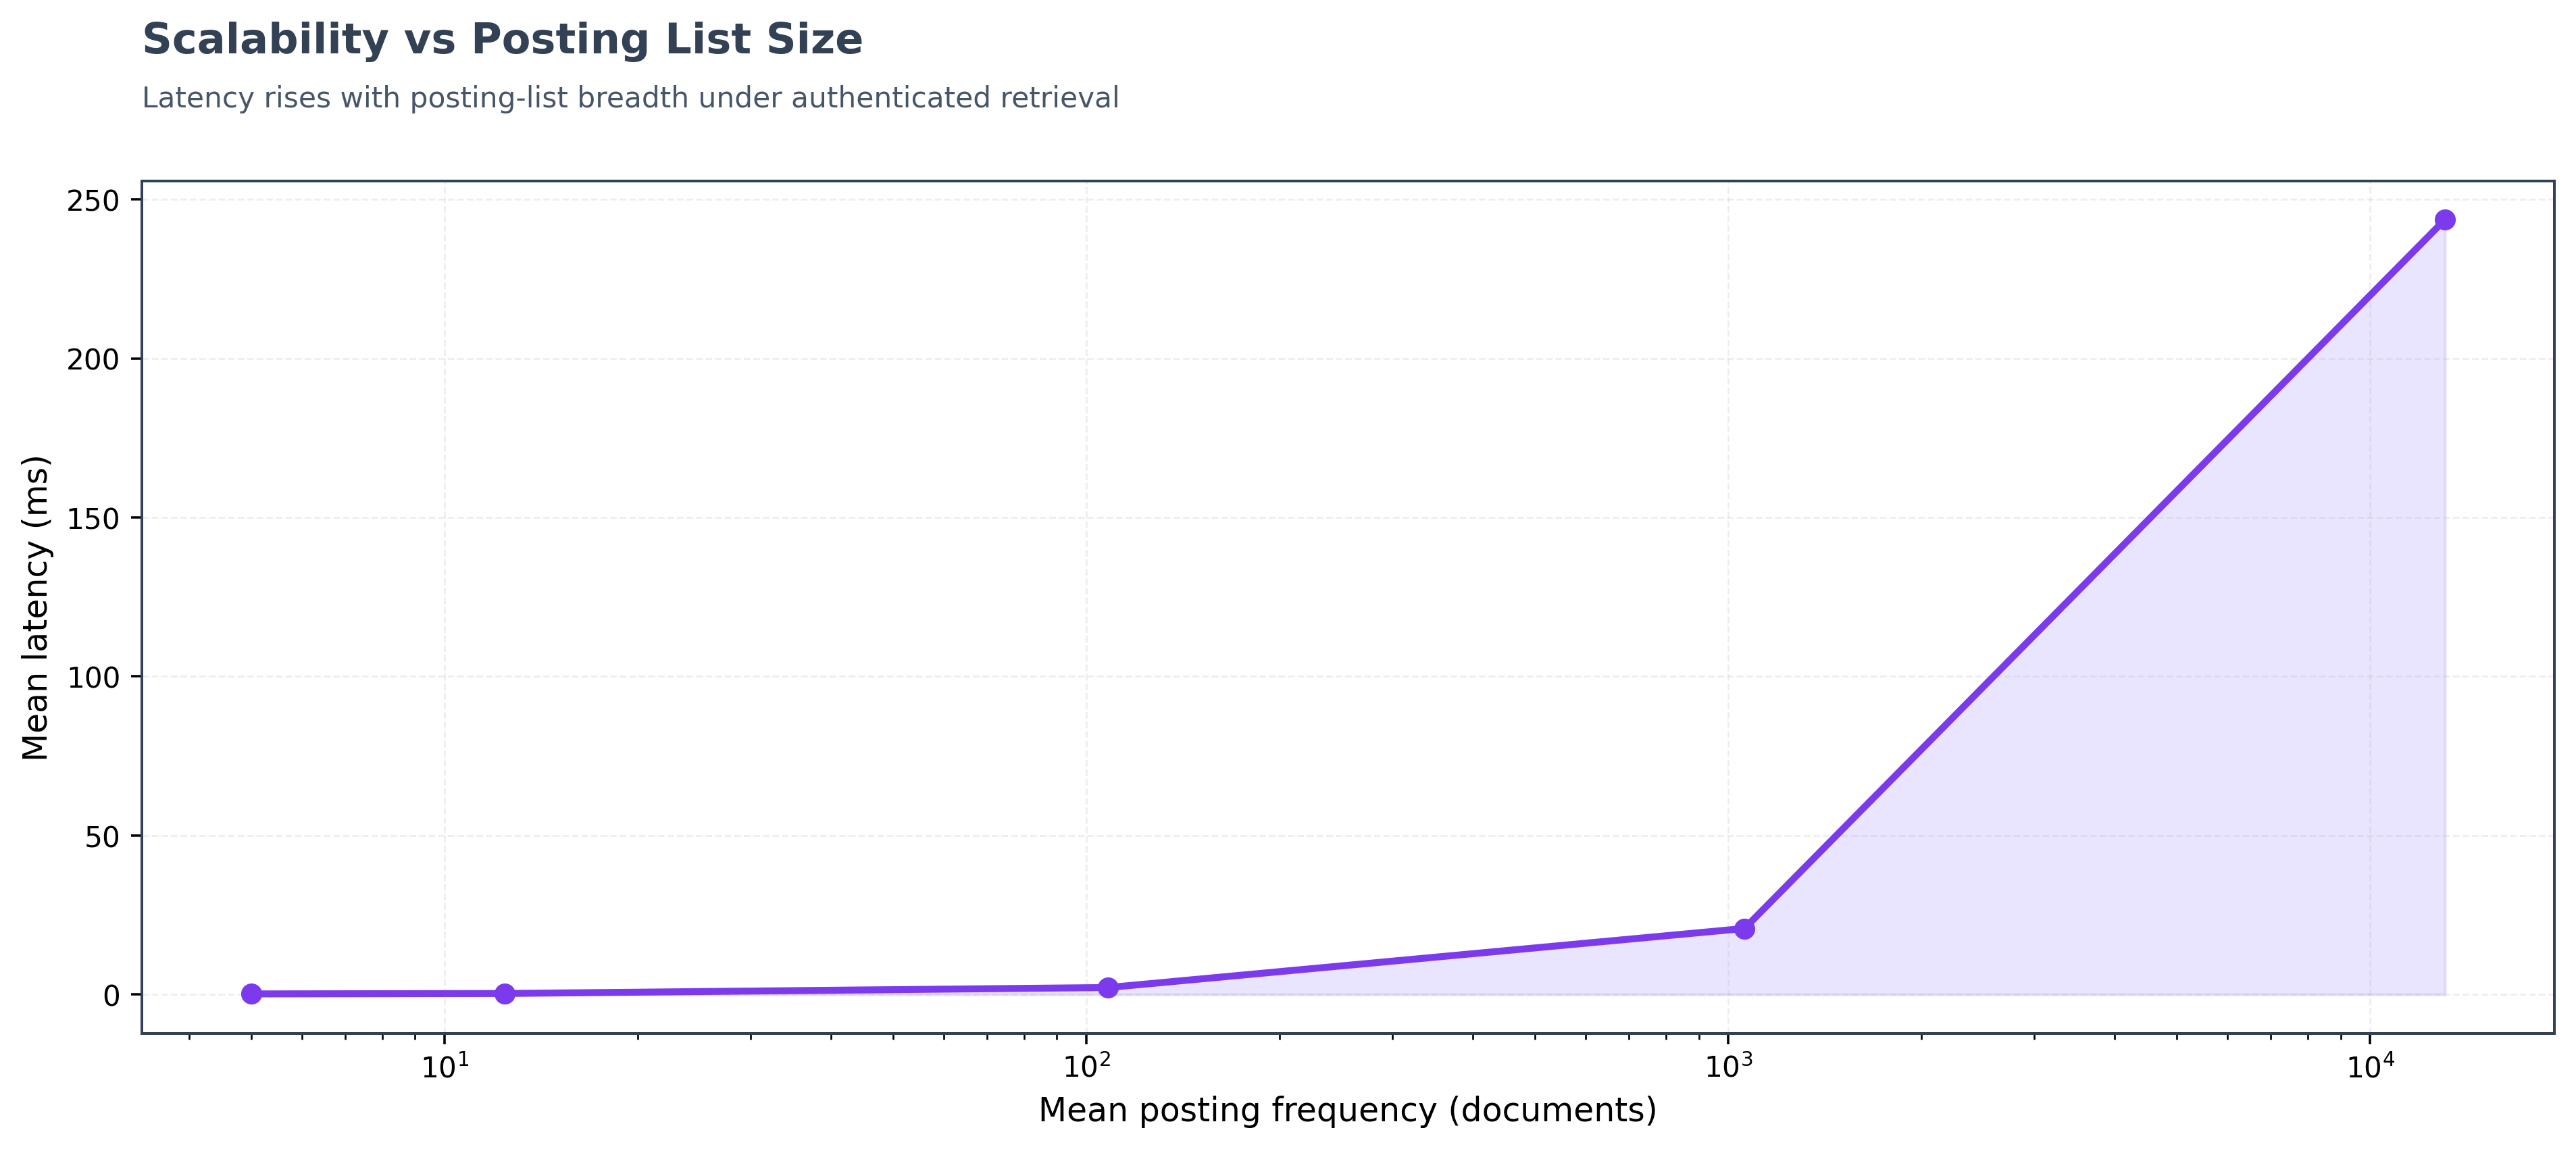
\includegraphics[width=\linewidth]{pics/figure_06_scalability_vs_posting_list_size.png}
\caption{Scalability with respect to posting-list size.}
\label{fig:scalepost}
\end{figure}
\begin{figure}[t]
\centering
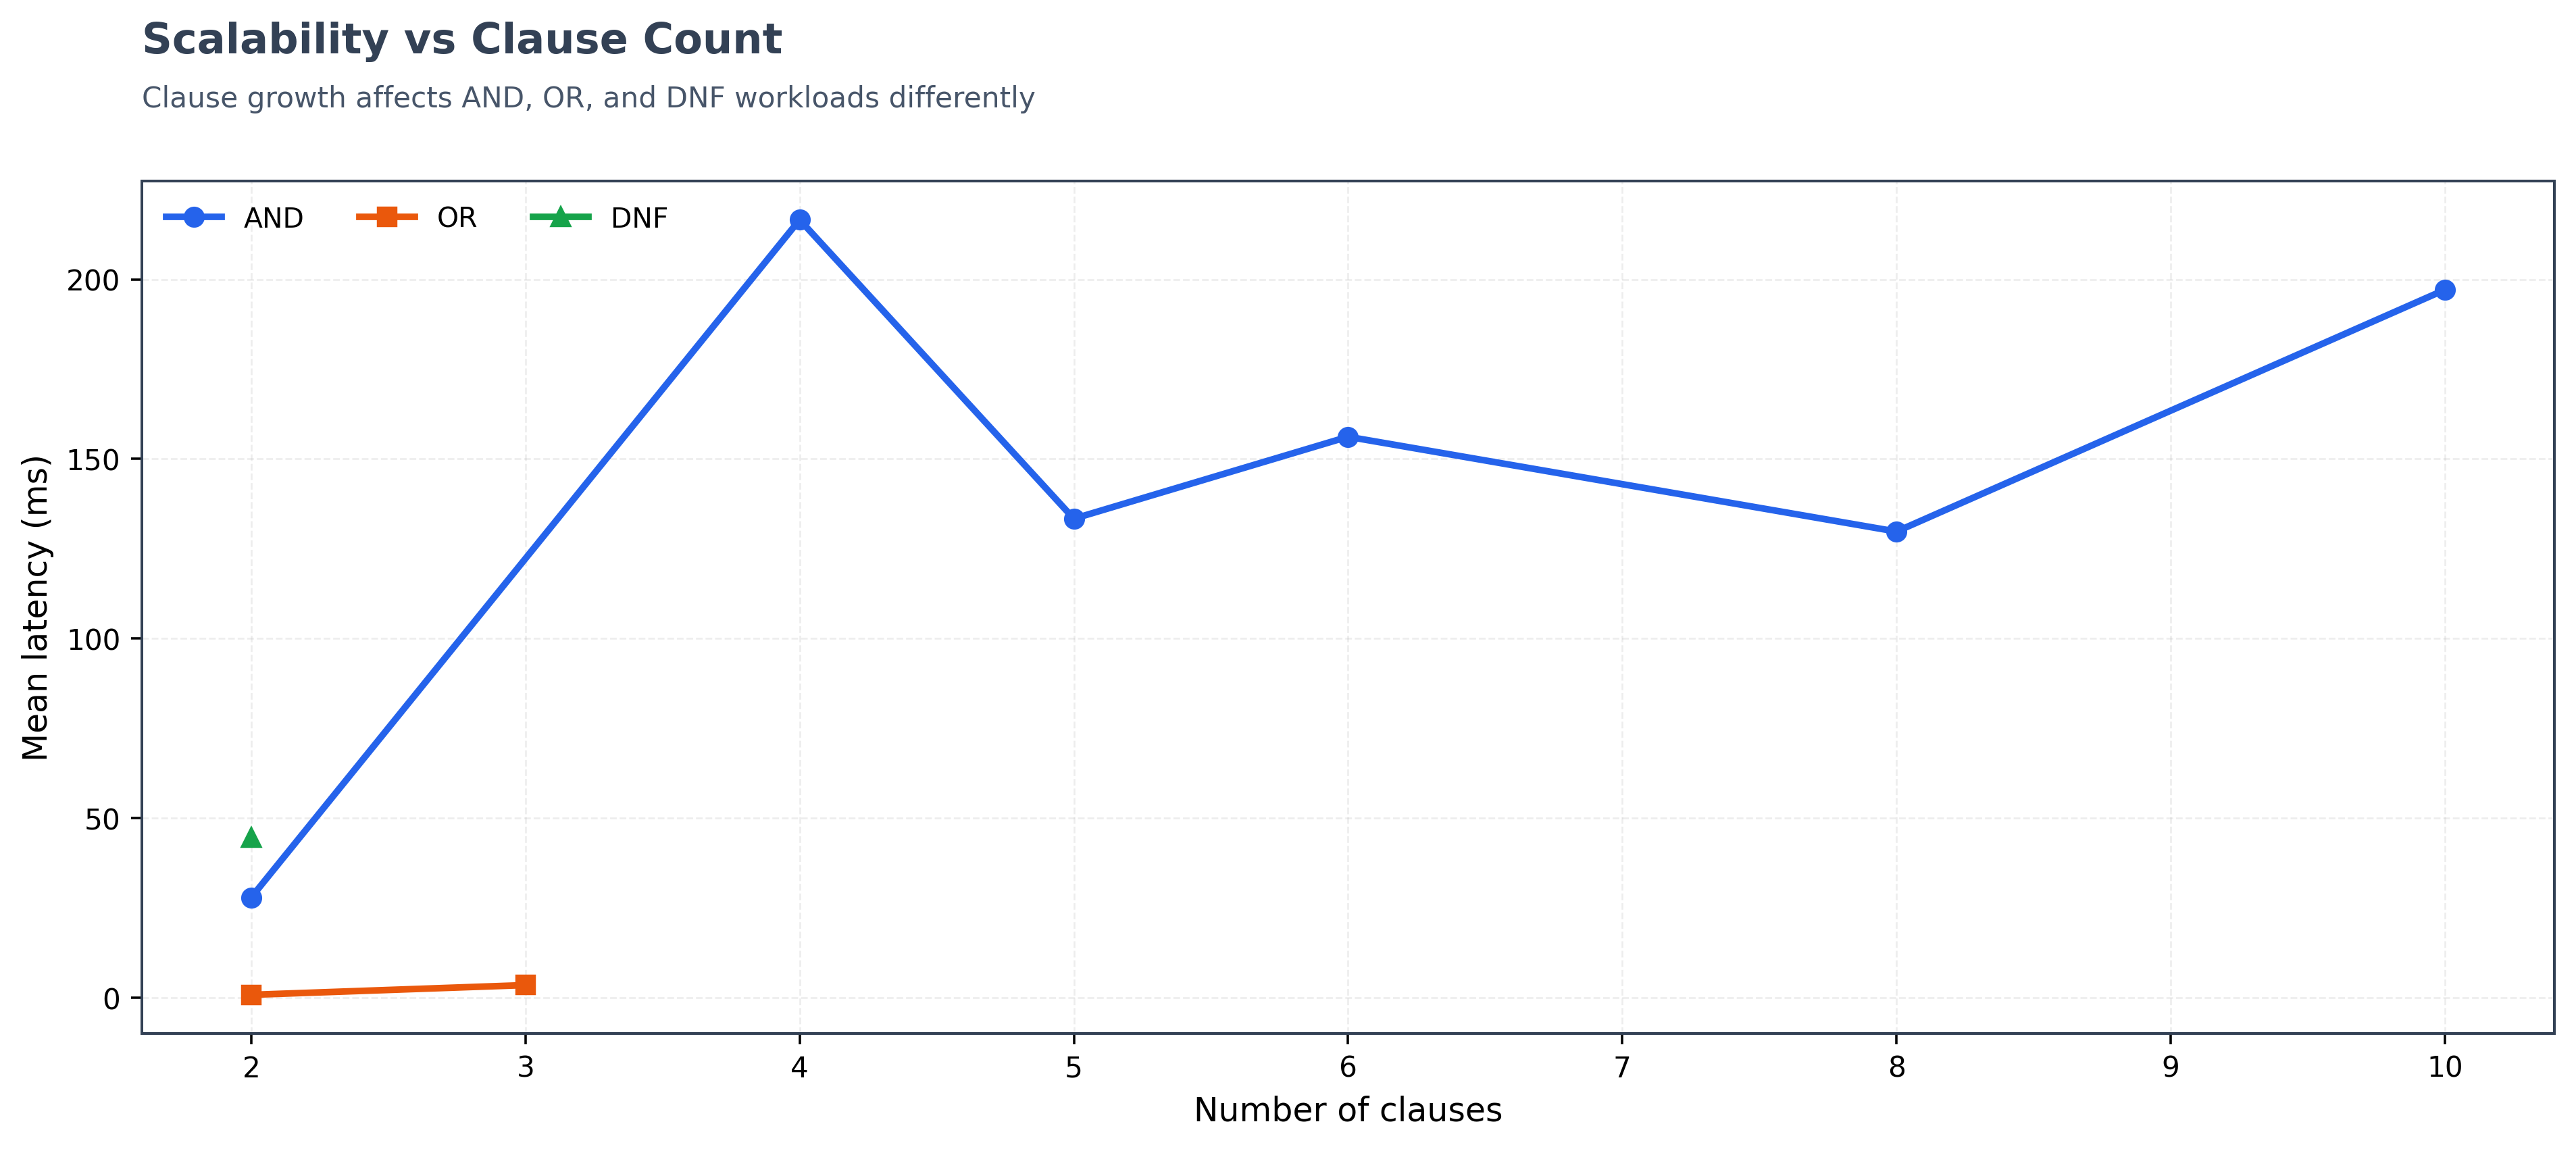
\includegraphics[width=\linewidth]{pics/figure_07_scalability_vs_clause_count.png}
\caption{Scalability with respect to clause count across conjunctive, disjunctive, and DNF query modes.}
\label{fig:scaleclause}
\end{figure}
\begin{figure}[t]
\centering
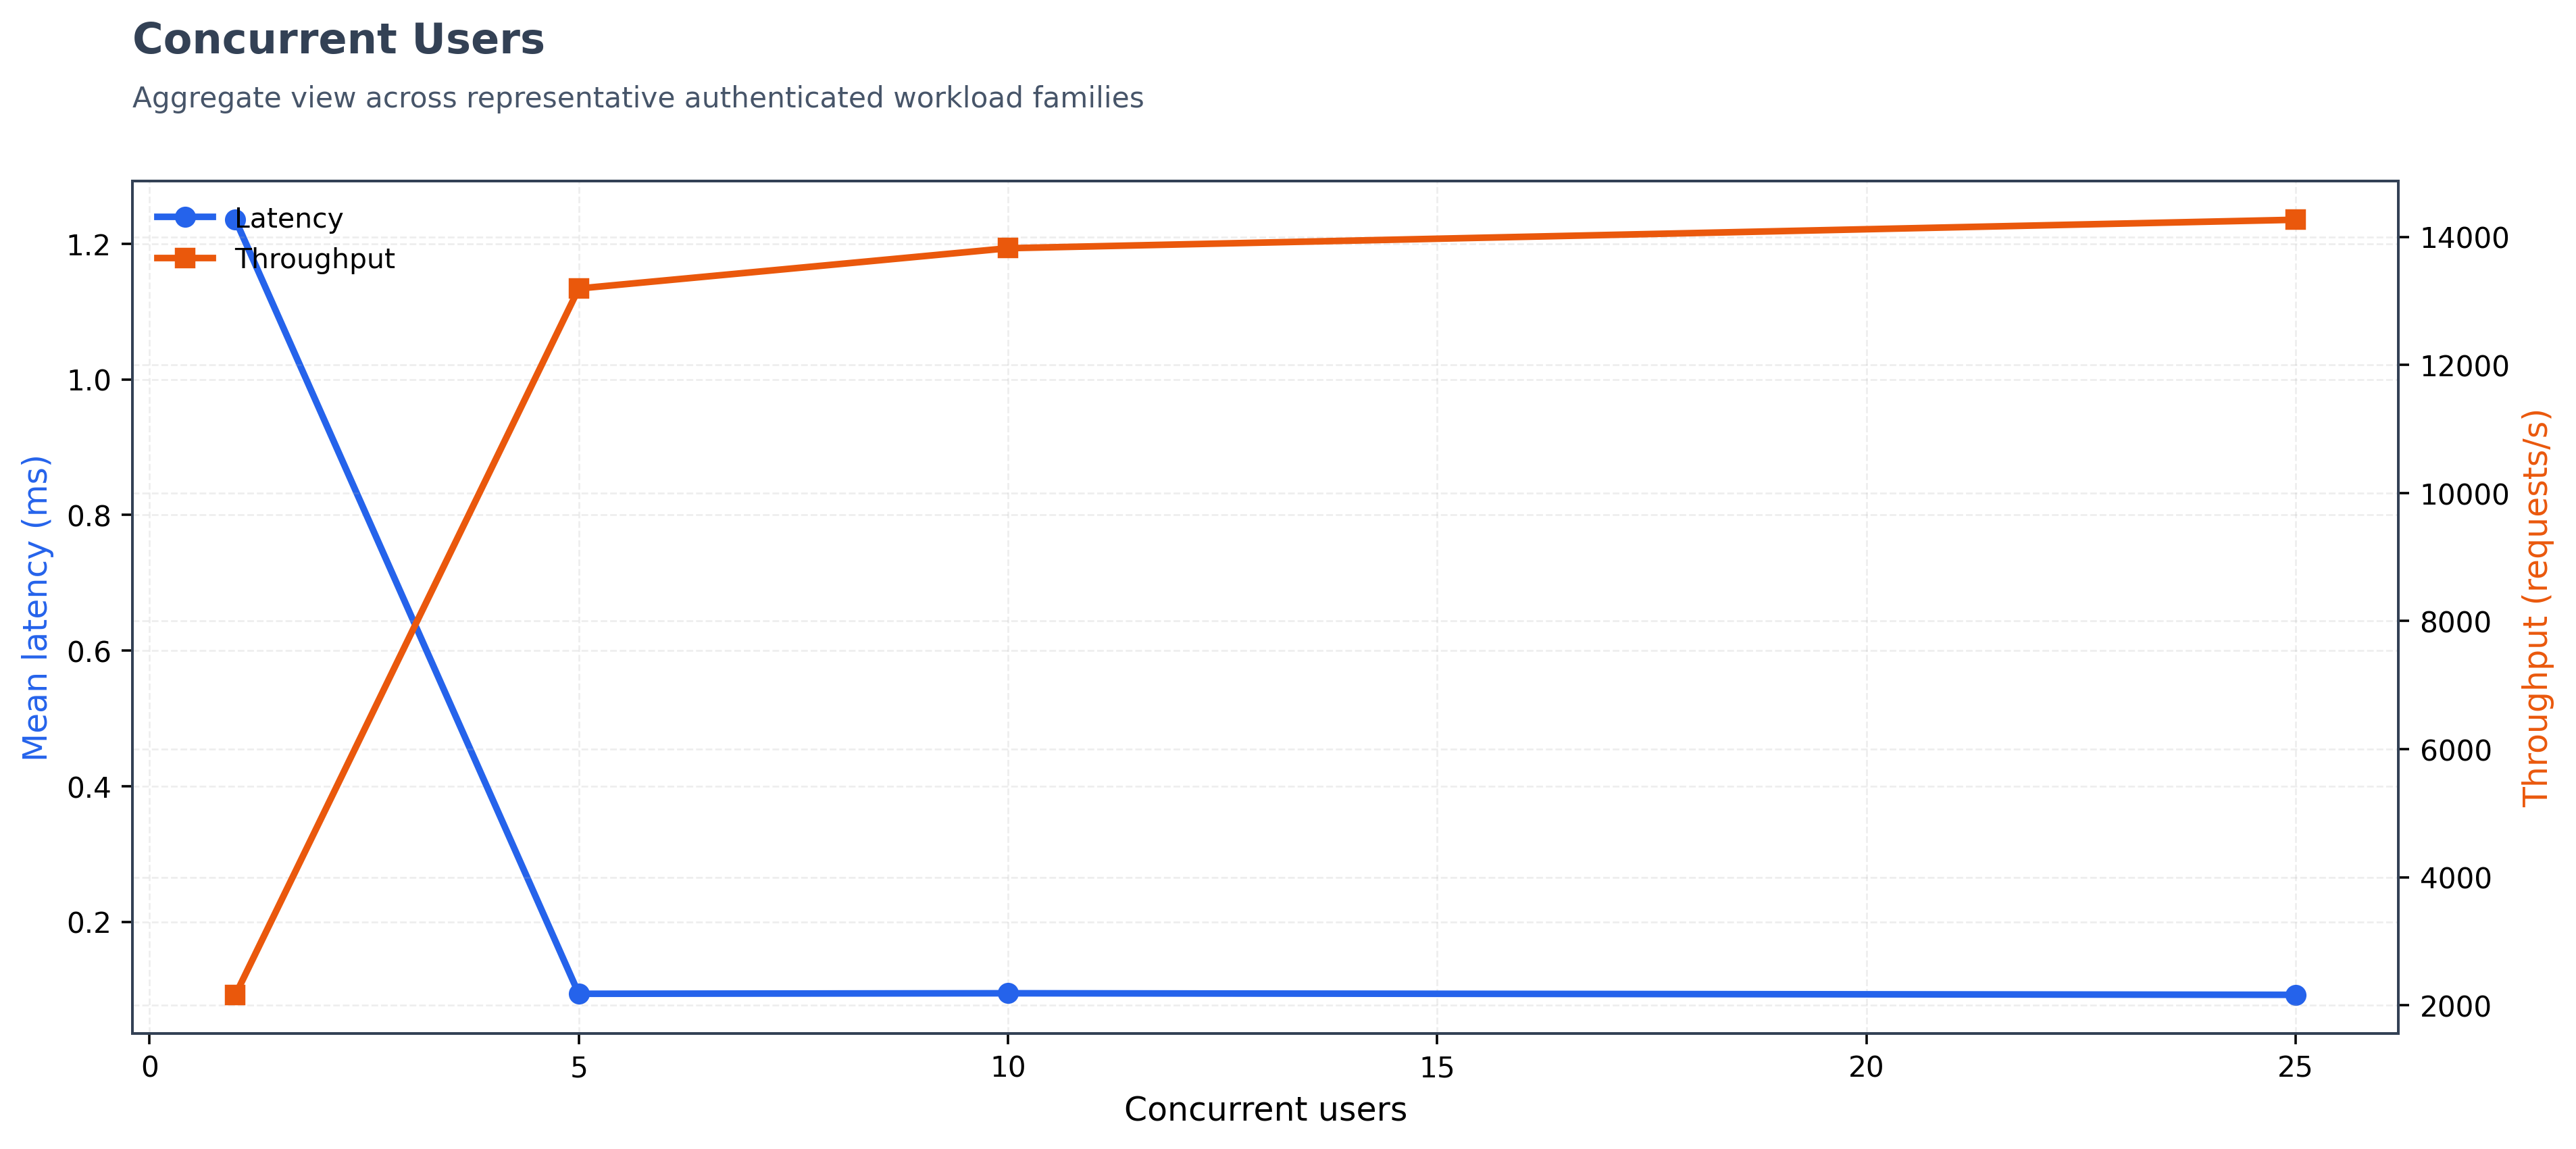
\includegraphics[width=\linewidth]{pics/figure_08_concurrent_users.png}
\caption{Throughput and latency under concurrent request load; success rate remains 100.00\% at all tested concurrency levels.}
\label{fig:concurrency}
\end{figure}
\subsection{Replay-Protection Results}
\label{4N}
The replay benchmark (Table~\ref{tab:replay}, Fig.~\ref{fig:replay}) directly operationalizes Theorem~5: it accepted all 200 first requests and rejected all 200 replayed requests, a 100.00\% replay-rejection rate, with mean rejection latency of 0.8019~ms and P95 rejection latency of 1.2123~ms, matching the $O(1)$ replay-check cost of Corollary~3. This closes a gap identified in the prior hybrid-blockchain evidence underlying this work, where replay attempts were previously detectable only through after-the-fact audit inspection rather than rejected in real time at the API boundary.
\begin{table}[t]
\centering
\caption{Replay-Protection Results}
\label{tab:replay}
\small
\begin{tabular}{lr}
\toprule
\textbf{Metric} & \textbf{Value} \\
\midrule
Attempted & 200 \\
Accepted first requests & 200 \\
Replayed requests rejected & 200 \\
Replay rejection rate & 100.00\% \\
Mean replay-rejection latency & 0.8019 ms \\
P95 replay-rejection latency & 1.2123 ms \\
\bottomrule
\end{tabular}
\end{table}
\begin{figure}[t]
\centering
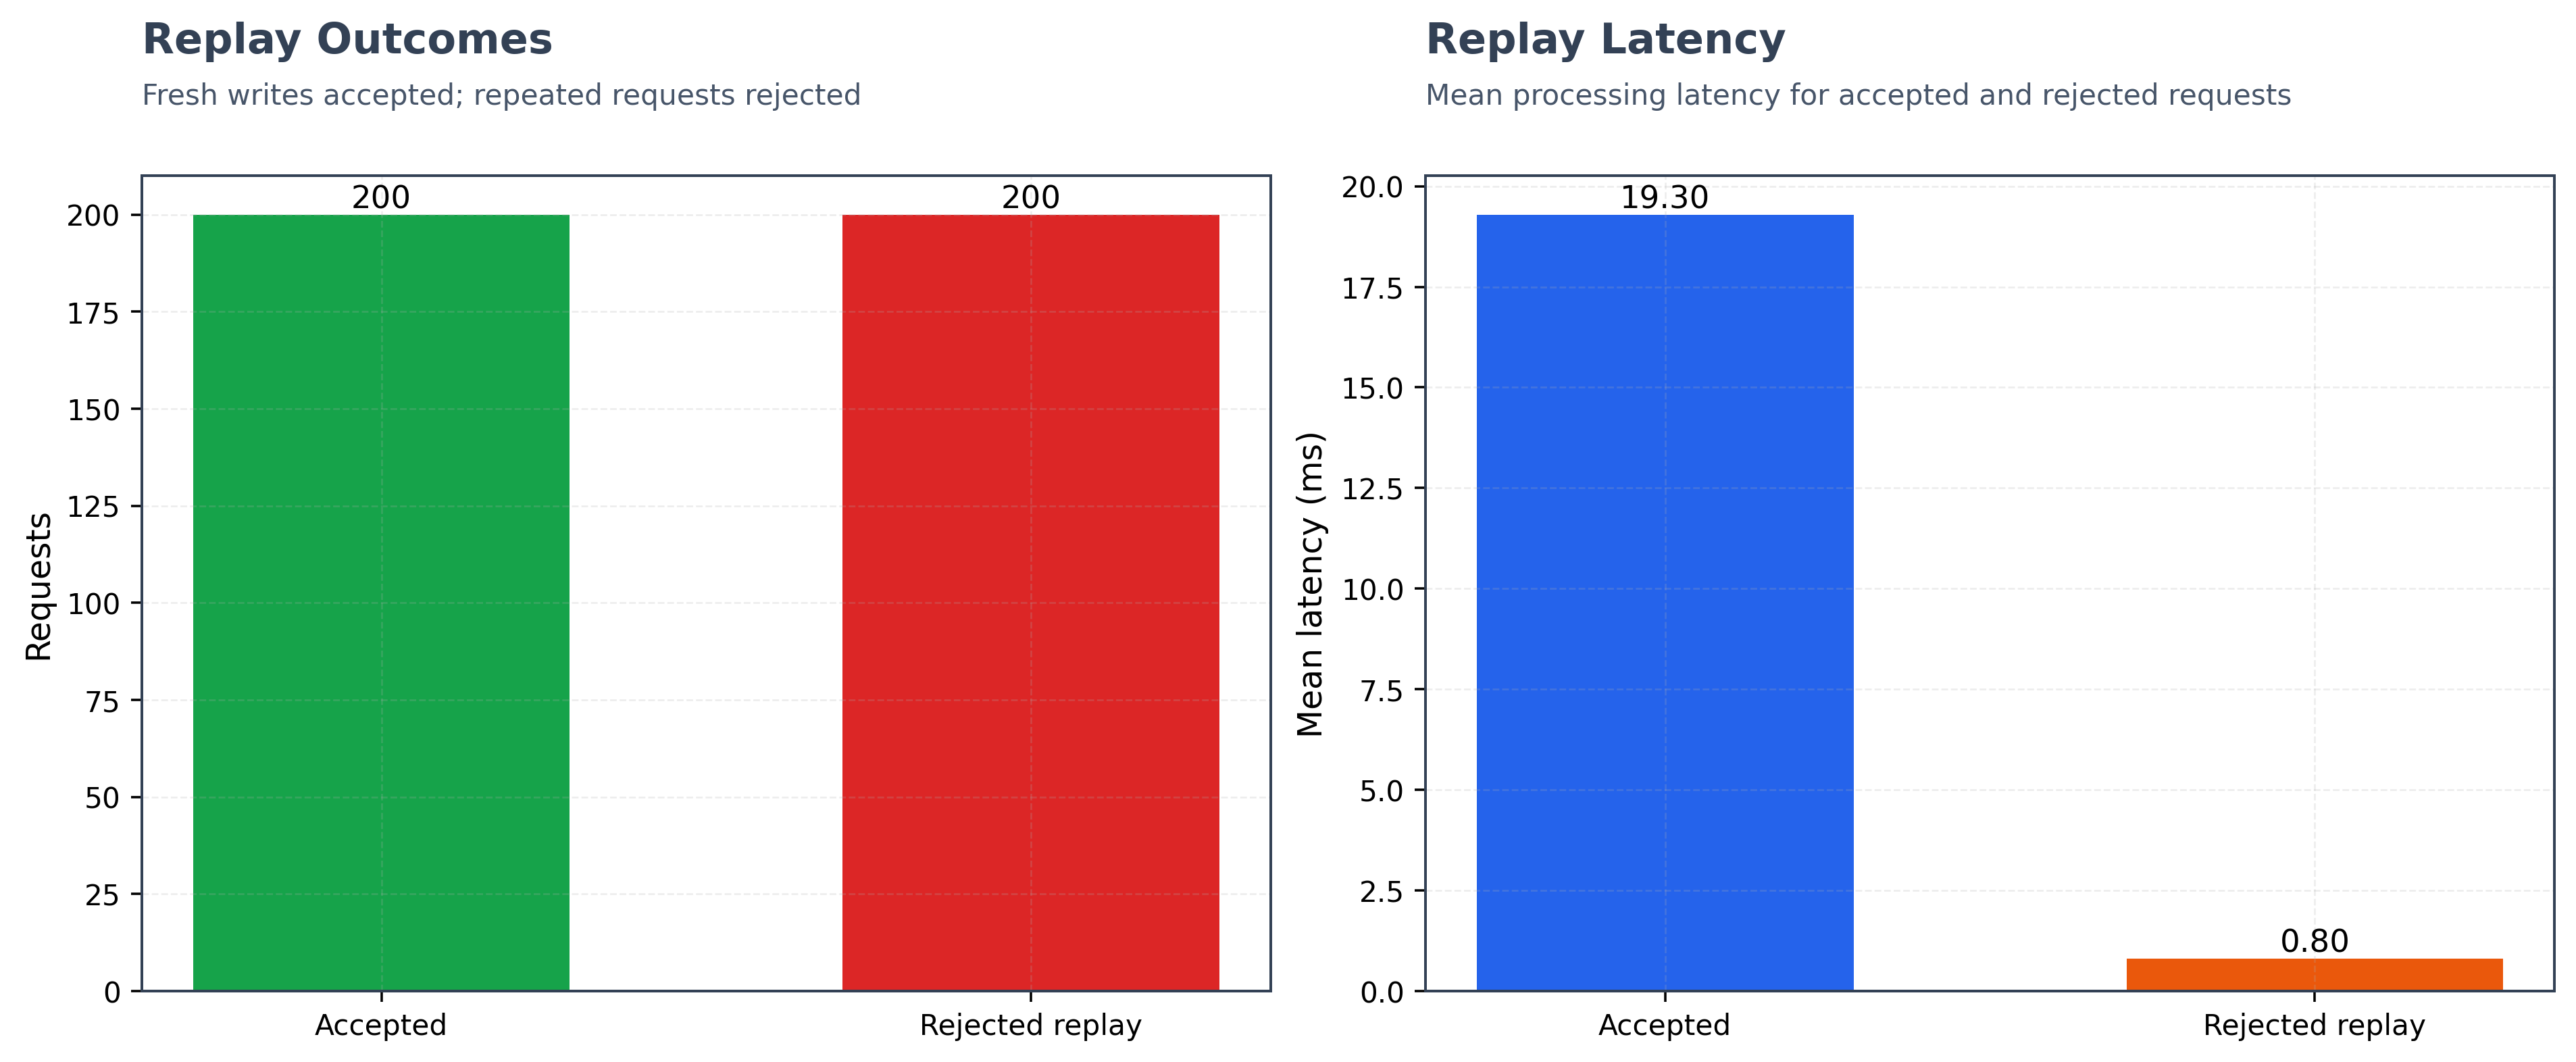
\includegraphics[width=\linewidth]{pics/figure_05_replay_protection_benchmark.png}
\caption{Replay-protection benchmark: acceptance of first requests versus rejection of replayed requests, and rejection-latency distribution.}
\label{fig:replay}
\end{figure}
\subsection{WAN-Style Distributed Validation}
\label{4O}
A distributed-validation benchmark starts real local HTTP validator peers and imposes LAN, regional-WAN, and cross-site-WAN latency and jitter profiles across 2, 4, 7, and 10 nodes. All configurations achieved 100.00\% success. Fig.~\ref{fig:distval} shows end-to-end threshold-path and full-signature-path latency across the matrix; under the cross-site-WAN profile at 10 nodes, the threshold path averaged 95.6609~ms end-to-end versus 120.5883~ms for the full-signature path, supporting the design choice to favor threshold collection over all-node confirmation when bounded validation latency is required. This benchmark is stronger than a no-network validator-overhead experiment because signatures are collected over real HTTP peer interactions under injected latency and jitter; it does not, however, include independently hosted, geographically separated machines or public-network routing, and is therefore reported as WAN-style distributed-validation evidence rather than a completed multi-site physical deployment (Section~\ref{sec:conclusion}).

\begin{figure}[t]
\centering
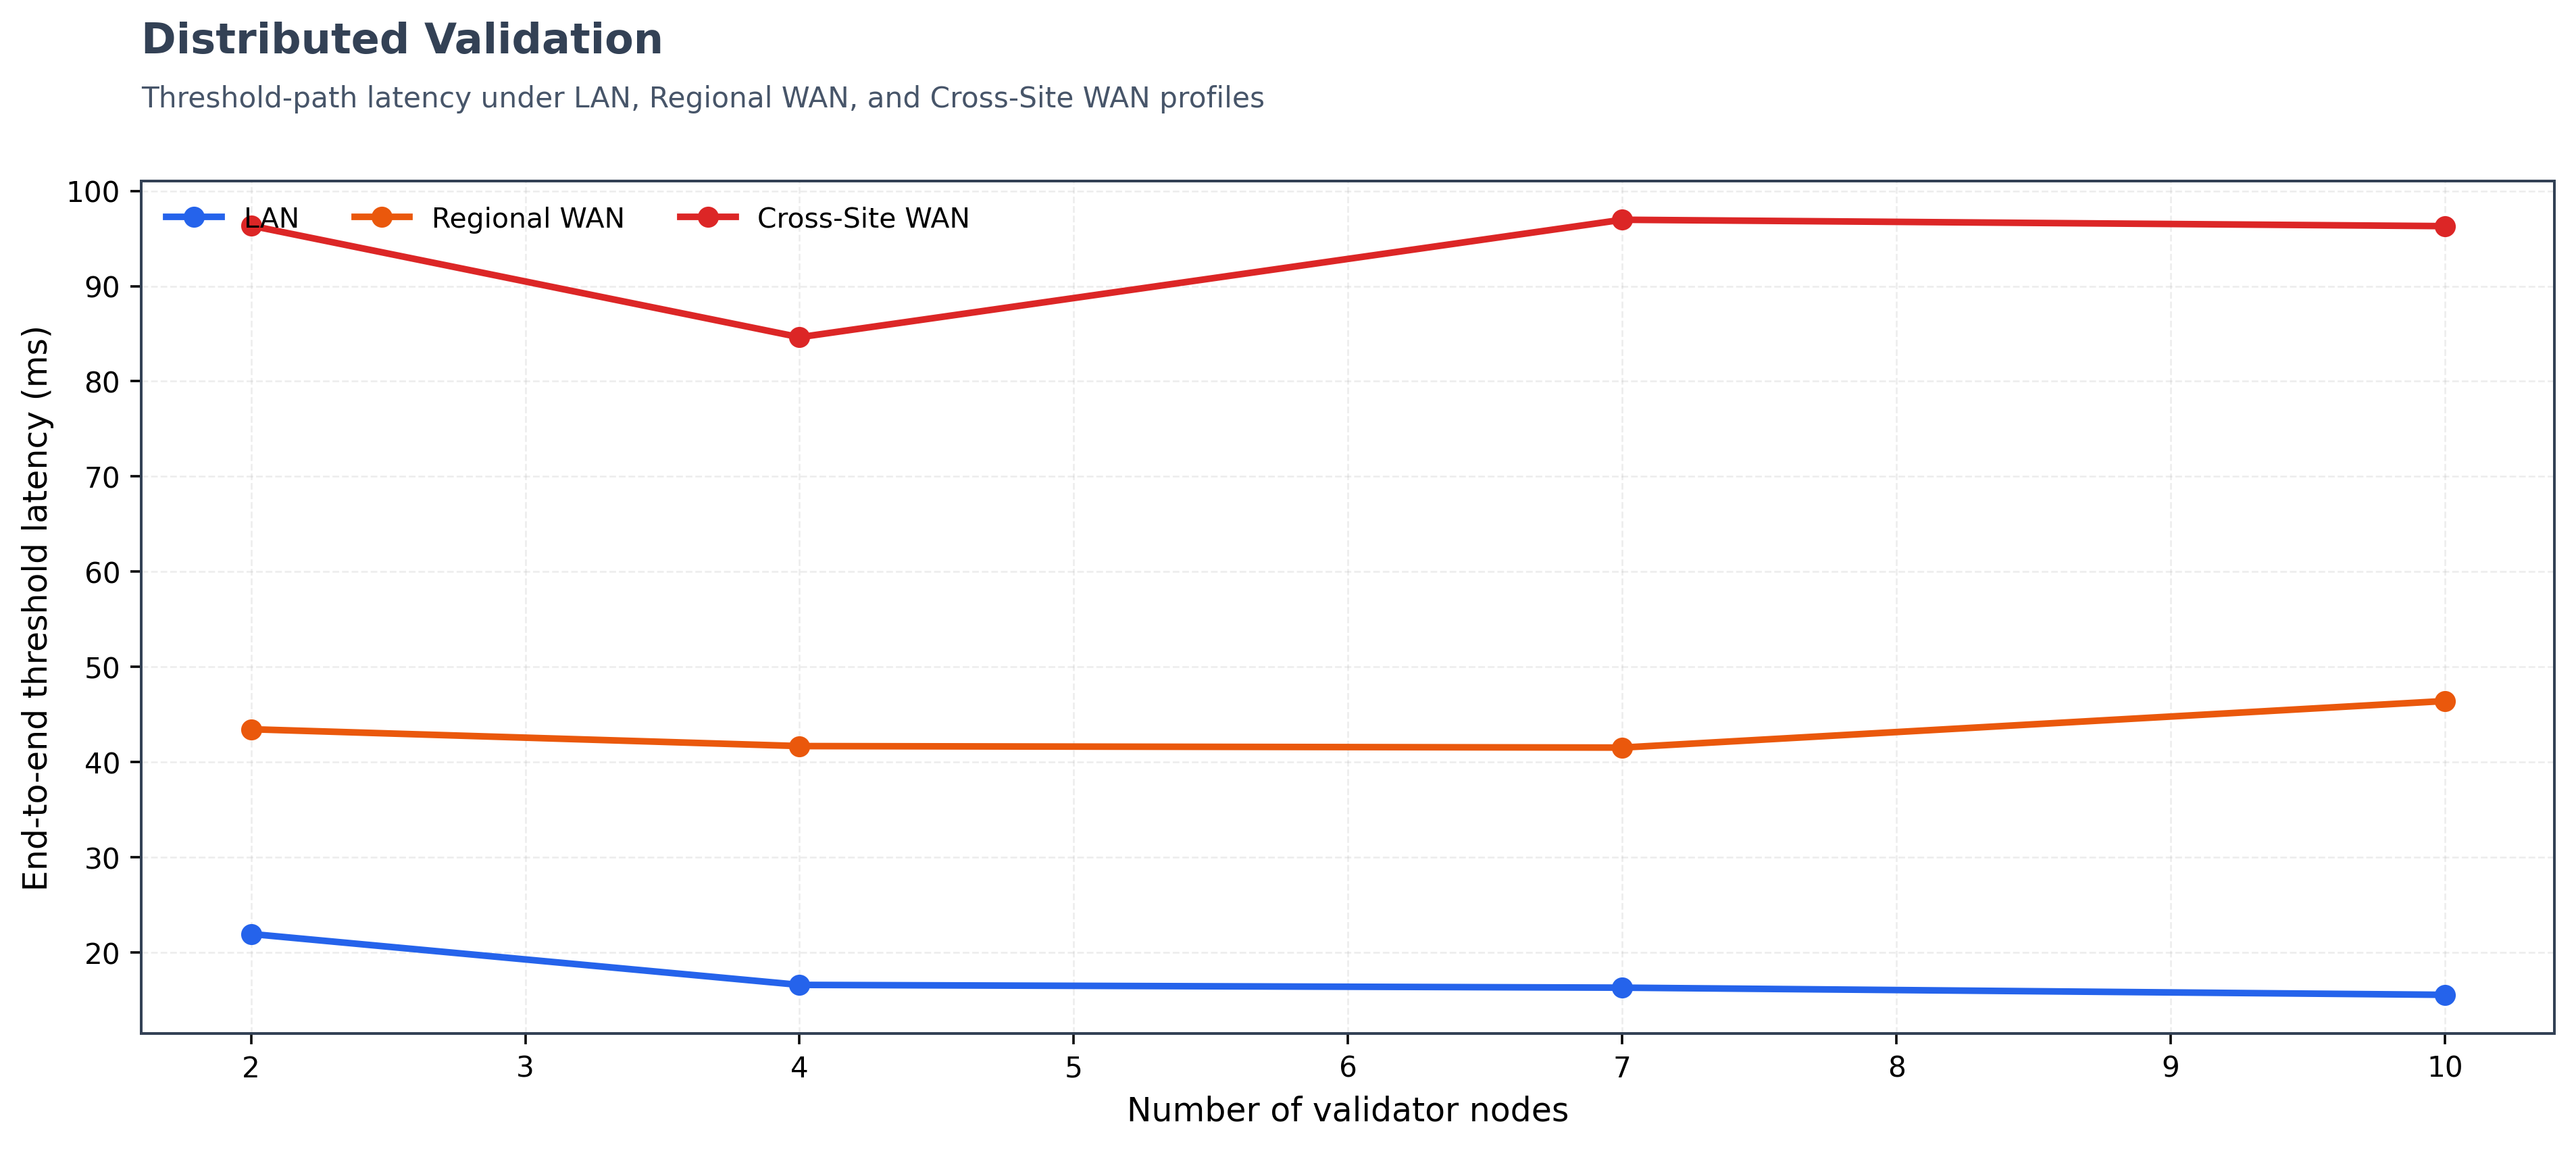
\includegraphics[width=\linewidth]{pics/figure_06_wan_style_distributed_validation.png}
\caption{WAN-style distributed-validation latency across LAN, regional-WAN, and cross-site-WAN profiles for 2, 4, 7, and 10 validator nodes.}
\label{fig:distval}
\end{figure}
\subsection{Discussion}
\label{4P}
The evidence in Sections~\ref{4D}--~\ref{4O} supports three manuscript-level claims. First, the extended query classes motivating PrivSearch authenticated OR, OR-of-AND, temporal range, fuzzy, and semantic-v1 search, together with real-time replay rejection are not only design proposals but executable, benchmarked prototype behavior with zero verification failures across 436 Enron-derived and 258 healthcare-derived workloads. Second, the dominant cost throughout the evaluation is authentication rather than raw search (78.59\%--80.57\% weighted share depending on corpus and family), which is the empirical signature of the latency-separation and cost-decomposition arguments of Section~III-F rather than an incidental implementation artifact. Third, the SeaCQ-aligned overlay shows substantial practical headroom under matched benchmark conditions while broadening the query language beyond conjunctive-only retrieval, and the broader literature-based comparison shows PrivSearch occupying a feature intersection encrypted query privacy, authenticated verification, richer post-conjunctive operators, and replay protection not simultaneously covered by TELEX, EAQ, VQL, or MSTDB.
At the same time, three deployment-relevant scenarios illustrate practical relevance without overstating maturity. In hospitals, PrivSearch supports authenticated low-latency retrieval across heterogeneous record collections while preserving auditability through the hybrid on-/off-chain design of Section~\ref{3A}. In pharmaceutical supply chains, authenticated OR and range queries are particularly useful for provenance tracing and recall investigation when multiple alternative identifiers or temporal windows must be searched, and the replay-protection layer guards against duplicated audit-submission replays. In cross-institution data-sharing settings, the authenticated-query model reduces reliance on a single remote administrator and supports verifiable retrieval across partially trusted organizations, which the 281,042-record, three-source healthcare validation directly supports. Full production deployment across geographically separated institutions and continuously operating IoMT infrastructures nonetheless remains future systems work beyond the present single-environment prototype evidence, consistent with the scope boundary stated in Section~IV-C and revisited in Section~\ref{sec:conclusion}.
